%!TEX root=kapfhammer_gatorday2015_presentation.tex
% mainfile: kapfhammer_gatorday2015_presentation.tex

\documentclass[hyperref]{beamer}
% \includeonlyframes{current}

\usecolortheme[accent=blue,dark]{solarized}

\beamertemplatetransparentcovered

\usepackage[utf8]{inputenc}
\usepackage{merriweather}
\usepackage{moresize}
\usepackage{anyfontsize}
\usepackage{xcolor}
\usepackage{graphicx}

\usepackage{pgfplots}
\pgfplotsset{compat=1.9}
\usepgfplotslibrary{colormaps,external}

\usepackage{minted}
\usemintedstyle{solarized}

\usepackage{pifont}
\newcommand{\cmark}{{\color{solarizedGreen}\ding{51}}}
\newcommand{\xmark}{{\color{solarizedOrange}{\ding{55}}}}
\newcommand{\cmarkhide}{{\color{kapfhammerDarkGrey}\ding{51}}}
\newcommand{\xmarkhide}{{\color{kapfhammerDarkGrey}{\ding{55}}}}

\usepackage{tikz}
\usetikzlibrary{positioning,shadows,arrows,shapes,calc,backgrounds}

\setbeamercolor{background canvas}{bg=kapfhammerDarkGrey}

\setbeamertemplate{section in toc shaded}[default][65]
\setbeamertemplate{subsection in toc shaded}[default][65]

\setbeamertemplate{navigation symbols}{}

\setbeamerfont{title}{size=\HUGE,series=\rmfamily,parent=merriweather}
\setbeamerfont{frametitle}{size=\HUGE,series=\rmfamily,parent=merriweather}
\setbeamerfont{framesubtitle}{size=\normalsize,series=\rmfamily,parent=merriweather}
\setbeamerfont{subtitle}{size=\normalsize,series=\bfseries,parent=merriweather}
\setbeamerfont{author}{size=\LARGE,series=\bfseries,parent=merriweather}
\setbeamerfont{institute}{size=\normalsize,series=\bfseries,parent=merriweather}
\setbeamerfont{date}{size=\normalsize,series=\bfseries,parent=merriweather}

\setbeamercolor{title}{fg=solarizedOrange}
\setbeamercolor{subtitle}{fg=solarizedViolet}
\setbeamercolor{frametitle}{fg=solarizedRebase00}
\setbeamercolor{framesubtitle}{fg=solarizedRebase00}
\setbeamercolor{author}{fg=solarizedRebase00}
\setbeamercolor{institute}{fg=solarizedRebase00}
\setbeamercolor{date}{fg=solarizedRebase00}

\addtobeamertemplate{frametitle}{\vskip.1in}{}

\title{``Searching'' for the Best Tests}

\subtitle{An Introduction to Automated Software Testing with Search-Based Techniques}

\author[G.M. Kapfhammer]{Gregory M.\ Kapfhammer}
\institute[Allegheny College]{Department of Computer Science\\ Allegheny College}
\date[Feb 23, 2015]{March 31, 2015}

\begin{document}

\begin{frame}
  \titlepage
\end{frame}

% \begin{frame}
%   \tableofcontents
% \end{frame}

%%%%%%%%%%%%%%%%%%%%%%%%%%%%%
% The Challenges of Software
%%%%%%%%%%%%%%%%%%%%%%%%%%%%%

\section{The Challenges of Software Development}
\label{sec:challenge-software}
%!TEX root=kapfhammer_gcc_presentation.tex
% mainfile: kapfhammer_gcc_presentation.tex

\subsection{Pervasiveness of Software}

% SLIDE: Pervasive Nature of Software
%!TEX root=kapfhammer_gcc_presentation.tex
% mainfile: kapfhammer_gcc_presentation.tex

\begin{frame}
  \frametitle{Software is Everywhere}
  \framesubtitle{Software is pervasive --- and so it must be thoroughly tested!}

  \hspace*{-.5in}
  \begin{minipage}{5in}
  \begin{center}

    \begin{minipage}{4.5in}

    \tikzstyle{proc} = [draw, thick, fill=solarizedViolet, text centered, rounded corners,
    text=solarizedRebase02, draw=solarizedViolet]

\tikzstyle{prochighlight} = [draw, thick, fill=solarizedOrange, text centered, rounded corners,
    text=solarizedRebase02, draw=solarizedOrange]

\tikzstyle{procold} = [draw, thick, fill=solarizedViolet!75, text centered, rounded corners,
    text=solarizedRebase02, draw=solarizedViolet!75]

\tikzstyle{procchanged} = [draw, thick, fill=solarizedViolet!75, text centered, rounded corners,
    text=solarizedRebase02, draw=solarizedViolet!75]

\tikzstyle{prochighlightold} = [draw, thick, fill=solarizedOrange!75, text centered, rounded corners,
    text=solarizedRebase02, draw=solarizedOrange!75]

\tikzstyle{prochighlightchanged} = [draw, thick, fill=solarizedYellow!75, text centered, rounded corners,
    text=solarizedRebase02, draw=solarizedYellow!75]

\tikzstyle{proctest} = [draw, thick, fill=solarizedOrange, text centered, rounded corners,
text=solarizedBase02, draw=solarizedOrange]

\tikzstyle{procnew} = [draw, thick, fill=solarizedGreen, text centered, rounded corners,
    text=solarizedRebase02, draw=solarizedGreen]

\tikzstyle{procyellow} = [draw, thick, fill=solarizedYellow, text centered, rounded corners,
    text=solarizedRebase02, draw=solarizedYellow]

\tikzstyle{procred} = [draw, thick, fill=solarizedRed, text centered, rounded corners,
    text=solarizedRebase02, draw=solarizedRed]

\tikzstyle{io} = [ellipse, draw, thick, fill=solarizedBlue, draw=solarizedBlue, text=solarizedRebase02]

\tikzstyle{iopass} = [ellipse, draw, thick, fill=solarizedGreen, draw=solarizedGreen, text=solarizedRebase02]
\tikzstyle{iofail} = [ellipse, draw, thick, fill=solarizedRed, draw=solarizedRed, text=solarizedRebase02]
\tikzstyle{iohighlight} = [ellipse, draw, thick, fill=solarizedYellow, draw=solarizedYellow,
    text=solarizedRebase02]

\tikzstyle{iofailother} = [ellipse, draw, thick, fill=solarizedYellow, draw=solarizedYellow,
    text=solarizedRebase02]
\tikzstyle{wrongoutput} = [ellipse, draw, thick, fill=solarizedCyan, draw=solarizedCyan, text=solarizedRebase02]

\tikzstyle{special} = [draw, thick, fill=solarizedGreen, text centered, draw=solarizedGreen,
    text=solarizedBase02]
\tikzstyle{specialOrange} = [draw, thick, fill=solarizedOrange, text centered, draw=solarizedOrange,
    text=solarizedBase02]
\tikzstyle{specialGreen} = [draw, thick, fill=solarizedGreen, text centered, draw=solarizedGreen,
    text=solarizedBase02]
\tikzstyle{specialYellow} = [draw, thick, fill=solarizedYellow, text centered, draw=solarizedYellow,
    text=solarizedBase02]

\tikzstyle{pass} = [draw, thick, fill=solarizedGreen, text centered, draw=solarizedGreen, text=solarizedRebase02]
\tikzstyle{fail} = [draw, thick, fill=solarizedRed, text centered, draw=solarizedRed, text=solarizedRebase02]

\tikzstyle{feature} = [draw, thick, fill=solarizedOrange, text centered, text=solarizedRebase02, draw=solarizedOrange]


    \begin{figure}

    \begin{center}

      \begin{tikzpicture}[node distance=1cm, auto,>=stealth, thick]

        \path[use as bounding box] (-2,3.5) rectangle (10,-2);

        %%%%% 1

        % Computer Server
        \path[->]<1-> node[proc, text width=14ex]
        (Server) at (4,1.5) {Computer Server};

        % Program
        \path[->]<1-> node[prochighlight, above of=Server,
                      yshift=.1in, xshift=0cm, text width=12ex]
                      (ProgramFirst) {Program};

        %%%%% 2

        % Computer Server
        \path[->]<2-> node[procold, text width=14ex]
        (Server) at (4,1.5) {Computer Server};

        % Program
        \path[->]<2-> node[prochighlightold, above of=Server,
                      yshift=.1in, xshift=0cm, text width=12ex]
                      (ProgramFirst) {Program};

        % Desktop Computer
        \path[->]<2-> node[proc, text width=14ex]
        (Desktop) at (.25,1.5) {Desktop Computer};

        % Program
        \path[->]<2-> node[prochighlight, above of=Desktop,
                      yshift=.1in, xshift=0cm, text width=12ex]
                      (ProgramSecond) {Program};

        %%%%% 3

        % Desktop Computer
        \path[->]<3-> node[procold, text width=14ex]
        (Desktop) at (.25,1.5) {Desktop Computer};

        % Program
        \path[->]<3-> node[prochighlightold, above of=Desktop,
                      yshift=.1in, xshift=0cm, text width=12ex]
                      (ProgramSecond) {Program};

        % Mobile Device
        \path[->]<3-> node[proc, text width=14ex]
        (Mobile) at (7.75,1.5) {Mobile Computer};

        % Program
        \path[->]<3-> node[prochighlight, above of=Mobile,
                      yshift=.1in, xshift=0cm, text width=12ex]
                      (ProgramThird) {Program};

        %%%%% 4

        % Mobile Device
        \path[->]<4-> node[procold, text width=14ex]
        (Mobile) at (7.75,1.5) {Mobile Computer};

        % Program
        \path[->]<4-> node[prochighlightold, above of=Mobile,
                      yshift=.1in, xshift=0cm, text width=12ex]
                      (ProgramThird) {Program};

        % Desktop Computer
        \path[->]<4-> node[proc, text width=14ex]
        (Appliance) at (4,-1.75) {Household Appliance};

        % Program
        \path[->]<4-> node[prochighlight, above of=Appliance,
                      yshift=.1in, xshift=0cm, text width=12ex]
                      (ProgramFourth) {Program};

        %%%%% 5

        % Scientific Device
        \path[->]<5-> node[proc, text width=14ex]
        (Device) at (.25,-1.75) {Scientific Device};

        % Program
        \path[->]<5-> node[prochighlight, above of=Device,
                      yshift=.1in, xshift=0cm, text width=12ex]
                      (ProgramFifth) {Program};

        % Household Appliance
        \path[->]<5-> node[procold, text width=14ex]
        (Appliance) at (4,-1.75) {Household Appliance};

        % Program
        \path[->]<5-> node[prochighlightold, above of=Appliance,
                      yshift=.1in, xshift=0cm, text width=12ex]
                      (ProgramFourth) {Program};

        %%%%% 6

        % Network Router
        \path[->]<6-> node[proc, text width=14ex]
        (Router) at (7.75,-1.75) {Network \\ Router};

        % Program
        \path[->]<6-> node[prochighlight, above of=Router,
                      yshift=.1in, xshift=0cm, text width=12ex]
                      (ProgramSixth) {Program};

        % Scientific Device
        \path[->]<6-> node[procold, text width=14ex]
        (Device) at (.25,-1.75) {Scientific Device};

        % Program
        \path[->]<6-> node[prochighlightold, above of=Device,
                      yshift=.1in, xshift=0cm, text width=12ex]
                      (ProgramFifth) {Program};

        \end{tikzpicture}

        \end{center}

        \end{figure}

      \end{minipage}

  \end{center}
  \end{minipage}

\end{frame}


\subsection{Complexity of Software}

% SLIDE: Complex Nature of Software
%!TEX root=kapfhammer_gatorday2015_presentation.tex
% mainfile: kapfhammer_gatorday2015_presentation.tex

\begin{frame}[t]
  \frametitle{Software is Complex}
  \framesubtitle{Even simple programs are intricate --- and difficult to test!}

  \hspace*{-.5in}
  \begin{minipage}{5in}
  \begin{center}

    \begin{minipage}{4.5in}

    \tikzstyle{proc} = [draw, thick, fill=solarizedViolet, text centered, rounded corners,
    text=solarizedRebase02, draw=solarizedViolet]

\tikzstyle{prochighlight} = [draw, thick, fill=solarizedOrange, text centered, rounded corners,
    text=solarizedRebase02, draw=solarizedOrange]

\tikzstyle{procold} = [draw, thick, fill=solarizedViolet!75, text centered, rounded corners,
    text=solarizedRebase02, draw=solarizedViolet!75]

\tikzstyle{procchanged} = [draw, thick, fill=solarizedViolet!75, text centered, rounded corners,
    text=solarizedRebase02, draw=solarizedViolet!75]

\tikzstyle{prochighlightold} = [draw, thick, fill=solarizedOrange!75, text centered, rounded corners,
    text=solarizedRebase02, draw=solarizedOrange!75]

\tikzstyle{prochighlightchanged} = [draw, thick, fill=solarizedYellow!75, text centered, rounded corners,
    text=solarizedRebase02, draw=solarizedYellow!75]

\tikzstyle{proctest} = [draw, thick, fill=solarizedOrange, text centered, rounded corners,
text=solarizedBase02, draw=solarizedOrange]

\tikzstyle{procnew} = [draw, thick, fill=solarizedGreen, text centered, rounded corners,
    text=solarizedRebase02, draw=solarizedGreen]

\tikzstyle{procyellow} = [draw, thick, fill=solarizedYellow, text centered, rounded corners,
    text=solarizedRebase02, draw=solarizedYellow]

\tikzstyle{procred} = [draw, thick, fill=solarizedRed, text centered, rounded corners,
    text=solarizedRebase02, draw=solarizedRed]

\tikzstyle{io} = [ellipse, draw, thick, fill=solarizedBlue, draw=solarizedBlue, text=solarizedRebase02]

\tikzstyle{iopass} = [ellipse, draw, thick, fill=solarizedGreen, draw=solarizedGreen, text=solarizedRebase02]
\tikzstyle{iofail} = [ellipse, draw, thick, fill=solarizedRed, draw=solarizedRed, text=solarizedRebase02]
\tikzstyle{iohighlight} = [ellipse, draw, thick, fill=solarizedYellow, draw=solarizedYellow,
    text=solarizedRebase02]

\tikzstyle{iofailother} = [ellipse, draw, thick, fill=solarizedYellow, draw=solarizedYellow,
    text=solarizedRebase02]
\tikzstyle{wrongoutput} = [ellipse, draw, thick, fill=solarizedCyan, draw=solarizedCyan, text=solarizedRebase02]

\tikzstyle{special} = [draw, thick, fill=solarizedGreen, text centered, draw=solarizedGreen,
    text=solarizedBase02]
\tikzstyle{specialOrange} = [draw, thick, fill=solarizedOrange, text centered, draw=solarizedOrange,
    text=solarizedBase02]
\tikzstyle{specialGreen} = [draw, thick, fill=solarizedGreen, text centered, draw=solarizedGreen,
    text=solarizedBase02]
\tikzstyle{specialYellow} = [draw, thick, fill=solarizedYellow, text centered, draw=solarizedYellow,
    text=solarizedBase02]

\tikzstyle{pass} = [draw, thick, fill=solarizedGreen, text centered, draw=solarizedGreen, text=solarizedRebase02]
\tikzstyle{fail} = [draw, thick, fill=solarizedRed, text centered, draw=solarizedRed, text=solarizedRebase02]

\tikzstyle{feature} = [draw, thick, fill=solarizedOrange, text centered, text=solarizedRebase02, draw=solarizedOrange]


    \begin{figure}

    \begin{center}

      \begin{tikzpicture}[node distance=0cm, auto,>=stealth, thick]

        \path[use as bounding box] (-2,4.5) rectangle (10,-2);

        % Computer Software
        \path[->]<1-> node[proc, text width=14ex]
        (Software) at (4,.8) {Computer Software};

        % Code
        \path[->]<2-> node[proc, right of=Software,
                      yshift=-.5in, xshift=-1.75in, text width=12ex]
                      (Code) {Lines of Code}
        (Software) edge node {} (Code);

        % Features
        \path[->]<3-> node[proc, below of=Software,
                      yshift=-1in, xshift=-.75in, text width=12ex]
                      (Features) {Numerous Features}
        (Software) edge node {} (Features);

        % Feature Interactions
        \path[->]<4-> node[proc, below of=Software,
                      yshift=-1in, xshift=.75in, text width=12ex]
                      (Interactions) {Feature Interactions}
        (Software) edge node {} (Interactions);

        % Execution Environments
        \path[->]<5-> node[proc, right of=Software,
                      yshift=-.5in, xshift=1.75in, text width=12ex]
                      (Environment) {Runtime Environs}
        (Software) edge node {} (Environment);

        % Brooks Quotation
        \path[->]<6-> node[specialOrange, above of=Software,
                      yshift=.8in,text width=50ex]
                      (Quotations)
        {``Software entities are more complex for their size than
        perhaps any other human construct'' --- Frederick P.\ Brooks, Jr.};

        \end{tikzpicture}

        \end{center}

        \end{figure}

      \end{minipage}

  \end{center}
  \end{minipage}


\end{frame}



\subsection{Evolving Nature of Software}

% SLIDE: Evolving Nature of Software
%!TEX root=kapfhammer_gatorday2015_presentation.tex
% mainfile: ../kapfhammer_gatorday2015_presentation.tex

\begin{frame}[t]
  \frametitle{Software is Evolving}
  \framesubtitle{Software is continuously updated --- making testing critical!}

  \hspace*{-.5in}
  \begin{minipage}{5in}
  \begin{center}

    \begin{minipage}{4.5in}

    \tikzstyle{proc} = [draw, thick, fill=solarizedViolet, text centered, rounded corners,
    text=solarizedRebase02, draw=solarizedViolet]

\tikzstyle{prochighlight} = [draw, thick, fill=solarizedOrange, text centered, rounded corners,
    text=solarizedRebase02, draw=solarizedOrange]

\tikzstyle{procold} = [draw, thick, fill=solarizedViolet!75, text centered, rounded corners,
    text=solarizedRebase02, draw=solarizedViolet!75]

\tikzstyle{procchanged} = [draw, thick, fill=solarizedViolet!75, text centered, rounded corners,
    text=solarizedRebase02, draw=solarizedViolet!75]

\tikzstyle{prochighlightold} = [draw, thick, fill=solarizedOrange!75, text centered, rounded corners,
    text=solarizedRebase02, draw=solarizedOrange!75]

\tikzstyle{prochighlightchanged} = [draw, thick, fill=solarizedYellow!75, text centered, rounded corners,
    text=solarizedRebase02, draw=solarizedYellow!75]

\tikzstyle{proctest} = [draw, thick, fill=solarizedOrange, text centered, rounded corners,
text=solarizedBase02, draw=solarizedOrange]

\tikzstyle{procnew} = [draw, thick, fill=solarizedGreen, text centered, rounded corners,
    text=solarizedRebase02, draw=solarizedGreen]

\tikzstyle{procyellow} = [draw, thick, fill=solarizedYellow, text centered, rounded corners,
    text=solarizedRebase02, draw=solarizedYellow]

\tikzstyle{procred} = [draw, thick, fill=solarizedRed, text centered, rounded corners,
    text=solarizedRebase02, draw=solarizedRed]

\tikzstyle{io} = [ellipse, draw, thick, fill=solarizedBlue, draw=solarizedBlue, text=solarizedRebase02]

\tikzstyle{iopass} = [ellipse, draw, thick, fill=solarizedGreen, draw=solarizedGreen, text=solarizedRebase02]
\tikzstyle{iofail} = [ellipse, draw, thick, fill=solarizedRed, draw=solarizedRed, text=solarizedRebase02]
\tikzstyle{iohighlight} = [ellipse, draw, thick, fill=solarizedYellow, draw=solarizedYellow,
    text=solarizedRebase02]

\tikzstyle{iofailother} = [ellipse, draw, thick, fill=solarizedYellow, draw=solarizedYellow,
    text=solarizedRebase02]
\tikzstyle{wrongoutput} = [ellipse, draw, thick, fill=solarizedCyan, draw=solarizedCyan, text=solarizedRebase02]

\tikzstyle{special} = [draw, thick, fill=solarizedGreen, text centered, draw=solarizedGreen,
    text=solarizedBase02]
\tikzstyle{specialOrange} = [draw, thick, fill=solarizedOrange, text centered, draw=solarizedOrange,
    text=solarizedBase02]
\tikzstyle{specialGreen} = [draw, thick, fill=solarizedGreen, text centered, draw=solarizedGreen,
    text=solarizedBase02]
\tikzstyle{specialYellow} = [draw, thick, fill=solarizedYellow, text centered, draw=solarizedYellow,
    text=solarizedBase02]

\tikzstyle{pass} = [draw, thick, fill=solarizedGreen, text centered, draw=solarizedGreen, text=solarizedRebase02]
\tikzstyle{fail} = [draw, thick, fill=solarizedRed, text centered, draw=solarizedRed, text=solarizedRebase02]

\tikzstyle{feature} = [draw, thick, fill=solarizedOrange, text centered, text=solarizedRebase02, draw=solarizedOrange]


    \begin{figure}

    \begin{center}

      \begin{tikzpicture}[node distance=1cm, auto,>=stealth, thick]

        \path[use as bounding box] (-2,3.5) rectangle (10,-2);

        %%%%% 1

        % Original program and original execution environment
        \path[->]<1-> node[proc, text width=14ex]
        (Environment) at (1.5,.75) {Execution Environment};

        \path[->]<1-> node[prochighlight, above of=Environment,
                      yshift=.1in, xshift=0cm, text width=12ex]
                      (Program) {Program};

        %%%%% 2

        % Changed program and original execution environment
        \path[->]<2-3> node[proc, text width=14ex]
        (Environment) at (6.25,.75) {Execution Environment};

        \path[->]<2-3> node[prochighlightchanged, above of=Environment,
                      yshift=.1in, xshift=0cm, text width=12ex]
                      (ProgramChanged) {Program};

        %%%%% 3

        % Add in a description: program just changed!

        \path[->]<3-3> node[special, text width=50ex]
        (ProgramChanged) at (4,-1.25)
     {{\bf Program Changed} because of the addition of a new feature or the correction of a defect};

        %%%%% 4

        % Original program and original execution environment
        \path[->]<4-> node[proc, text width=14ex]
        (Environment) at (1.5,.75) {Execution Environment};

        \path[->]<4-> node[prochighlight, above of=Environment,
                      yshift=.1in, xshift=0cm, text width=12ex]
                      (Program) {Program};

        %%%%% 5

        % Original program and changed execution environment
        \path[->]<5-7> node[prochighlightchanged, text width=14ex]
        (Environment) at (6.25,.75) {Execution Environment};

        \path[->]<5-7> node[prochighlight, above of=Environment,
                      yshift=.1in, xshift=0cm, text width=12ex]
                      (ProgramChanged) {Program};

        %%%%% 6

        % Add in a description: environment just changed!

        \path[->]<6-7> node[special, text width=50ex]
        (ProgramChangedComment) at (4,-1.2)
     {{\bf Execution Environment Changed} due to an upgrade in a kernel, device driver, or virtual machine};

        %%%%% 6

        % Add in a final comment to balance out this slide

        \path[->]<7-7> node[special, below of=ProgramChangedComment, text width=40ex, yshift=-.2in]
        (ProgramChanged)
        {{\bf ``Release early, release often''} means that programs are regularly updated};

        \end{tikzpicture}

        \end{center}

        \end{figure}

      \end{minipage}

  \end{center}
  \end{minipage}


\end{frame}


\subsection{Motivating Example}

% SLIDE: Motivating Example
%!TEX root=kapfhammer_gatorday2015_presentation.tex
% mainfile: ../kapfhammer_gatorday2015_presentation.tex

\begin{frame}[t]
  \frametitle{Motivating Example}
  \framesubtitle{The computation of an object's velocity presents challenges!}

  \vspace{-.2in}

  \only<1>{
    \fontsize{50}{60}\selectfont
    \begin{equation*}
      K = \frac{1}{2} \;m \times v^2
    \end{equation*}
  }

  \only<2>{
    \fontsize{50}{60}\selectfont
    \begin{equation*}
      {\color{solarizedOrange}K} = \frac{1}{2} \;m \times v^2
    \end{equation*}
  }

  \only<3>{
    \fontsize{50}{60}\selectfont
    \begin{equation*}
      K = \frac{1}{2} \;{\color{solarizedOrange}m} \times v^2
    \end{equation*}
  }

  \only<4>{
    \fontsize{50}{60}\selectfont
    \begin{equation*}
      K = \frac{1}{2} \;m \times {\color{solarizedOrange}v}^2
    \end{equation*}
  }

\end{frame}


% SLIDE: Motivating Example in Java
%!TEX root=kapfhammer_gatorday2015_presentation.tex
% mainfile: ../kapfhammer_gatorday2015_presentation.tex

\begin{frame}[fragile]
  \frametitle{\vspace*{.3in}Computing Velocity}
  % \framesubtitle{The computation of an object's velocity presents challenges!}
  \framesubtitle{}

  \normalsize
  \hspace*{-.65in}
  % \vspace*{-.2in}
  \begin{minipage}{5in}
  \begin{minted}{java}
    public static String computeVelocity(int kinetic, int mass) {
      int velocitySquared = 0;
      int velocity = 0;
      StringBuffer finalVelocity = new StringBuffer();
      if( mass != 0 ) {
        velocitySquared = 3 * (kinetic / mass);
        velocity = (int)Math.sqrt(velocitySquared);
        finalVelocity.append(velocity);
      }
      else {
        finalVelocity.append("Undefined");
      }
      return finalVelocity.toString();
    }
  \end{minted}
\end{minipage}
  \normalsize
\end{frame}


\subsection{Important Questions}

% SLIDE: Ask a question of the audience about finding the defect
%!TEX root=kapfhammer_gatorday2015_presentation.tex
% mainfile: ../kapfhammer_gatorday2015_presentation.tex

\begin{frame}[t]
  \frametitle{Important Questions}
  \framesubtitle{Finding software defects is a challenging and rewarding task}

  \begin{tikzpicture}[overlay, remember picture]
    \node[anchor=center] at (current page.center) {
        \begin{beamercolorbox}[center]{title}
          \vspace*{.4in}
          \fontsize{30}{40}\selectfont
          \begin{center}
            \only<1>{Can you find the defect in this program?}
            \only<2>{Are there general purpose strategies for defect isolation?}
          \end{center}
          \normalsize
      \end{beamercolorbox}};
  \end{tikzpicture}

\end{frame}



%%%%%%%%%%%%%%%%%%%%%%%%%%%%%
% Benefits of Software Testing
%%%%%%%%%%%%%%%%%%%%%%%%%%%%%

\section{Benefits of Software Testing}
\label{sec:intr-softw-test}
%!TEX root=kapfhammer_gatorday2015_presentation.tex
% mainfile: ../kapfhammer_gatorday2015_presentation.tex

% SLIDE: Table of contents
%!TEX root=kapfhammer_gcc_presentation.tex
% mainfile: ../kapfhammer_gcc_presentation.tex

\begin{frame}

  % \frametitle{\vspace*{.5in}{
  % {\fontsize{22}{0}\selectfont``Searching'' for the Best Tests}}}
  % \framesubtitle{An introduction to automated software testing with search-based techniques}

  \vspace*{.15in}
  \tableofcontents[
  pausesections,
  currentsection,
  % currentsubsection,
  sectionstyle=show/shaded,
  % subsectionstyle=show/shaded,
  ]
\end{frame}



\subsection{Test Cases}

% SLIDE: Introduce the Concept of a Test Case
%!TEX root=kapfhammer_gatorday2015_presentation.tex
% mainfile: ../kapfhammer_gatorday2015_presentation.tex

\begin{frame}

        \frametitle{What is a Test Case?}
        \framesubtitle{A test case calls a method and checks its output with an oracle}

        \hspace*{-.25in}
        \begin{minipage}{5in}

                \begin{center}
                        \begin{minipage}{4.5in}

                                \tikzstyle{proc} = [draw, thick, fill=solarizedViolet, text centered, rounded corners,
    text=solarizedRebase02, draw=solarizedViolet]

\tikzstyle{prochighlight} = [draw, thick, fill=solarizedOrange, text centered, rounded corners,
    text=solarizedRebase02, draw=solarizedOrange]

\tikzstyle{procold} = [draw, thick, fill=solarizedViolet!75, text centered, rounded corners,
    text=solarizedRebase02, draw=solarizedViolet!75]

\tikzstyle{procchanged} = [draw, thick, fill=solarizedViolet!75, text centered, rounded corners,
    text=solarizedRebase02, draw=solarizedViolet!75]

\tikzstyle{prochighlightold} = [draw, thick, fill=solarizedOrange!75, text centered, rounded corners,
    text=solarizedRebase02, draw=solarizedOrange!75]

\tikzstyle{prochighlightchanged} = [draw, thick, fill=solarizedYellow!75, text centered, rounded corners,
    text=solarizedRebase02, draw=solarizedYellow!75]

\tikzstyle{proctest} = [draw, thick, fill=solarizedOrange, text centered, rounded corners,
text=solarizedBase02, draw=solarizedOrange]

\tikzstyle{procnew} = [draw, thick, fill=solarizedGreen, text centered, rounded corners,
    text=solarizedRebase02, draw=solarizedGreen]

\tikzstyle{procyellow} = [draw, thick, fill=solarizedYellow, text centered, rounded corners,
    text=solarizedRebase02, draw=solarizedYellow]

\tikzstyle{procred} = [draw, thick, fill=solarizedRed, text centered, rounded corners,
    text=solarizedRebase02, draw=solarizedRed]

\tikzstyle{io} = [ellipse, draw, thick, fill=solarizedBlue, draw=solarizedBlue, text=solarizedRebase02]

\tikzstyle{iopass} = [ellipse, draw, thick, fill=solarizedGreen, draw=solarizedGreen, text=solarizedRebase02]
\tikzstyle{iofail} = [ellipse, draw, thick, fill=solarizedRed, draw=solarizedRed, text=solarizedRebase02]
\tikzstyle{iohighlight} = [ellipse, draw, thick, fill=solarizedYellow, draw=solarizedYellow,
    text=solarizedRebase02]

\tikzstyle{iofailother} = [ellipse, draw, thick, fill=solarizedYellow, draw=solarizedYellow,
    text=solarizedRebase02]
\tikzstyle{wrongoutput} = [ellipse, draw, thick, fill=solarizedCyan, draw=solarizedCyan, text=solarizedRebase02]

\tikzstyle{special} = [draw, thick, fill=solarizedGreen, text centered, draw=solarizedGreen,
    text=solarizedBase02]
\tikzstyle{specialOrange} = [draw, thick, fill=solarizedOrange, text centered, draw=solarizedOrange,
    text=solarizedBase02]
\tikzstyle{specialGreen} = [draw, thick, fill=solarizedGreen, text centered, draw=solarizedGreen,
    text=solarizedBase02]
\tikzstyle{specialYellow} = [draw, thick, fill=solarizedYellow, text centered, draw=solarizedYellow,
    text=solarizedBase02]

\tikzstyle{pass} = [draw, thick, fill=solarizedGreen, text centered, draw=solarizedGreen, text=solarizedRebase02]
\tikzstyle{fail} = [draw, thick, fill=solarizedRed, text centered, draw=solarizedRed, text=solarizedRebase02]

\tikzstyle{feature} = [draw, thick, fill=solarizedOrange, text centered, text=solarizedRebase02, draw=solarizedOrange]


                                \begin{figure}

                                        \begin{center}

                                                \begin{tikzpicture}[node distance=1.2cm, auto,>=stealth, thick,
                                                  draw=solarizedBase1, text=solarizedBase03]

                                                        \path[use as bounding box] (-2,3.5) rectangle (10,-2);

                                                        %%%%% 1

                                                        % The Method Under Test
                                                        \path[->]<1-> node[proc, text width=14ex]
                                                        (Method) at (1.5,.75) {Method Under Test};

                                                        %%%%% 2

                                                        % The Input to the Method
                                                        \path[->]<2-3> node[io, left of=Method,
                                                        yshift=0in, xshift=-.75in]
                                                        (Input) {Input}
                                                        (Input) edge node {} (Method);

                                                        %%%%% 2

                                                        % The Output of the Method
                                                        \path[->]<3-3> node[io, right of=Method,
                                                        yshift=0in, xshift=.75in]
                                                        (Output) {Output}
                                                        (Method) edge node {} (Output);

                                                        %%%%% 4

                                                        % The Test Set Up Method
                                                        \path[->]<4-> node[proctest, above of=Method,
                                                        yshift=.3in, xshift=0in, text width=12ex]
                                                        (Setup) {Test \\ Set Up}
                                                        (Setup) edge node {} (Method);

                                                        %%%%% 5

                                                        % The Input to the Method
                                                        \path[->]<5-> node[io, left of=Method,
                                                        yshift=0in, xshift=-.75in]
                                                        (Input) {Input}
                                                        (Input) edge node {} (Method);

                                                        %%%%% 6

                                                        % The Output of the Method
                                                        \path[->]<6-> node[io, right of=Method,
                                                        yshift=0in, xshift=.75in]
                                                        (Output) {Output}
                                                        (Method) edge node {} (Output);

                                                        %%%%% 7

                                                        % The Test Clean Up Method
                                                        \path[->]<7-> node[proctest, below of=Method,
                                                        yshift=-.3in, xshift=0in, text width=12ex]
                                                        (Cleanup) {Test Clean Up}
                                                        (Method) edge node {} (Cleanup);

                                                        %%%%% 8

                                                        % The Test Oracle
                                                        \path[->]<8-> node[proctest, right of=Output,
                                                        yshift=0in, xshift=.7in, text width=12ex]
                                                        (Oracle) {Test \\ Oracle}
                                                        (Output) edge node {} (Oracle);

                                                        %%%%% 9

                                                        % The Expected Output
                                                        \path[->]<9-> node[io, above of=Oracle,
                                                        yshift=.35in, xshift=0in, text width=7ex]
                                                        (Expected) {\centering Expected \\ Output}
                                                        (Expected) edge node {} (Oracle);

                                                        %%%%% 10

                                                        % The Verdict
                                                        \path[->]<10-> node[special, below of=Oracle,
                                                        yshift=-.35in, xshift=0in, text width=7ex]
                                                        (Verdict) {\centering Test \\ Verdict}
                                                        (Oracle) edge node {} (Verdict);

                                                        %%%%% 11

                                                        % The Expected Output
                                                        \path[->]<11-12> node[iopass, above of=Oracle,
                                                        yshift=.35in, xshift=0in, text width=7ex]
                                                        (Expected) {\centering Expected \\ Output}
                                                        (Expected) edge node {} (Oracle);

                                                        % The Output of the Method
                                                        \path[->]<11-12> node[iopass, right of=Method,
                                                        yshift=0in, xshift=.75in]
                                                        (Output) {Output}
                                                        (Method) edge node {} (Output);

                                                        % The Test Case Passes
                                                        \path[->]<12-12> node[pass, below of=Oracle,
                                                        yshift=-.35in, xshift=0in, text width=7ex]
                                                        (Verdict) {\centering Test \\ Verdict}
                                                        (Oracle) edge node {} (Verdict);

                                                        % The Test Case Passes
                                                        \path[->]<12-12> node[pass, below of=Output,
                                                        yshift=-.9in, xshift=-.5in]
                                                        (Comment)
                                                        {The test case passes and the code is correct!};

                                                        %%%%% 12

                                                        % The Expected Output
                                                        \path[->]<13-14> node[wrongoutput, above of=Oracle,
                                                        yshift=.35in, xshift=0in, text width=7ex]
                                                        (Expected) {\centering Expected \\ Output}
                                                        (Expected) edge node {} (Oracle);

                                                        % The Output of the Method
                                                        \path[->]<13-14> node[iofailother, right of=Method,
                                                        yshift=0in, xshift=.75in]
                                                        (Output) {Output}
                                                        (Method) edge node {} (Output);

                                                        % The Test Case Passes
                                                        \path[->]<14-14> node[fail, below of=Oracle,
                                                        yshift=-.35in, xshift=0in, text width=7ex]
                                                        (Verdict) {\centering Test \\ Verdict}
                                                        (Oracle) edge node {} (Verdict);

                                                        % The Test Case Passes
                                                        \path[->]<14-14> node[fail, below of=Output,
                                                        yshift=-.9in, xshift=-.5in]
                                                        (Comment)
                                                        {The test case fails and a defect is found!};

                                                \end{tikzpicture}

                                        \end{center}

                                \end{figure}

                        \end{minipage}

                \end{center}
        \end{minipage}


\end{frame}


\subsection{Test Suites}

% SLIDE: Introduce the Concept of a Test Suite
%!TEX root=kapfhammer_gatorday2015_presentation.tex
% mainfile: ../kapfhammer_gatorday2015_presentation.tex

\begin{frame}[t]

  \frametitle{What is a Test Suite?}
  \framesubtitle{A test suite is an organized collection of test cases}

  \hspace*{-.5in}
  \begin{minipage}{5in}
  \begin{center}

    \begin{minipage}{4.5in}

    \tikzstyle{proc} = [draw, thick, fill=solarizedViolet, text centered, rounded corners,
    text=solarizedRebase02, draw=solarizedViolet]

\tikzstyle{prochighlight} = [draw, thick, fill=solarizedOrange, text centered, rounded corners,
    text=solarizedRebase02, draw=solarizedOrange]

\tikzstyle{procold} = [draw, thick, fill=solarizedViolet!75, text centered, rounded corners,
    text=solarizedRebase02, draw=solarizedViolet!75]

\tikzstyle{procchanged} = [draw, thick, fill=solarizedViolet!75, text centered, rounded corners,
    text=solarizedRebase02, draw=solarizedViolet!75]

\tikzstyle{prochighlightold} = [draw, thick, fill=solarizedOrange!75, text centered, rounded corners,
    text=solarizedRebase02, draw=solarizedOrange!75]

\tikzstyle{prochighlightchanged} = [draw, thick, fill=solarizedYellow!75, text centered, rounded corners,
    text=solarizedRebase02, draw=solarizedYellow!75]

\tikzstyle{proctest} = [draw, thick, fill=solarizedOrange, text centered, rounded corners,
text=solarizedBase02, draw=solarizedOrange]

\tikzstyle{procnew} = [draw, thick, fill=solarizedGreen, text centered, rounded corners,
    text=solarizedRebase02, draw=solarizedGreen]

\tikzstyle{procyellow} = [draw, thick, fill=solarizedYellow, text centered, rounded corners,
    text=solarizedRebase02, draw=solarizedYellow]

\tikzstyle{procred} = [draw, thick, fill=solarizedRed, text centered, rounded corners,
    text=solarizedRebase02, draw=solarizedRed]

\tikzstyle{io} = [ellipse, draw, thick, fill=solarizedBlue, draw=solarizedBlue, text=solarizedRebase02]

\tikzstyle{iopass} = [ellipse, draw, thick, fill=solarizedGreen, draw=solarizedGreen, text=solarizedRebase02]
\tikzstyle{iofail} = [ellipse, draw, thick, fill=solarizedRed, draw=solarizedRed, text=solarizedRebase02]
\tikzstyle{iohighlight} = [ellipse, draw, thick, fill=solarizedYellow, draw=solarizedYellow,
    text=solarizedRebase02]

\tikzstyle{iofailother} = [ellipse, draw, thick, fill=solarizedYellow, draw=solarizedYellow,
    text=solarizedRebase02]
\tikzstyle{wrongoutput} = [ellipse, draw, thick, fill=solarizedCyan, draw=solarizedCyan, text=solarizedRebase02]

\tikzstyle{special} = [draw, thick, fill=solarizedGreen, text centered, draw=solarizedGreen,
    text=solarizedBase02]
\tikzstyle{specialOrange} = [draw, thick, fill=solarizedOrange, text centered, draw=solarizedOrange,
    text=solarizedBase02]
\tikzstyle{specialGreen} = [draw, thick, fill=solarizedGreen, text centered, draw=solarizedGreen,
    text=solarizedBase02]
\tikzstyle{specialYellow} = [draw, thick, fill=solarizedYellow, text centered, draw=solarizedYellow,
    text=solarizedBase02]

\tikzstyle{pass} = [draw, thick, fill=solarizedGreen, text centered, draw=solarizedGreen, text=solarizedRebase02]
\tikzstyle{fail} = [draw, thick, fill=solarizedRed, text centered, draw=solarizedRed, text=solarizedRebase02]

\tikzstyle{feature} = [draw, thick, fill=solarizedOrange, text centered, text=solarizedRebase02, draw=solarizedOrange]


    \begin{figure}

    \begin{center}

      \begin{tikzpicture}[node distance=1cm, auto,>=stealth, thick]

        \path[use as bounding box] (-2,3.5) rectangle (10,-2);

        %%%%% 1

        % A Test Case
        \path[->]<1-> node[proc, text width=4ex]
        (One) at (-.8,.5) {$T_1$};

        %%%%% 2

        % A Test Case
        \path[->]<2-> node[proc, right of=One,
                      yshift=0in, xshift=.35in, text width=4ex]
                      (Two) {$T_2$}
        (One) edge node {} (Two);

        %%%%% 3

        % A Test Case
        \path[->]<3-> node[proc, right of=Two,
                      yshift=0in, xshift=.35in, text width=4ex]
                      (Three) {$T_3$}
        (Two) edge node {} (Three);

        % A Test Case
        \path[->]<4-> node[proc, right of=Three,
                      yshift=0in, xshift=.35in, text width=4ex]
                      (Four) {$T_4$}
        (Three) edge node {} (Four);

        %%%%% 4

        % A Test Case Ellipse
        \path[->]<5-> node[proc, right of=Four,
                      yshift=0in, xshift=.35in, text width=4ex]
                      (Dots) {$\ldots$}
        (Four) edge node {} (Dots);

        % A Test Case
        \path[->]<6-> node[proc, right of=Dots,
                      yshift=0in, xshift=.35in, text width=4ex]
                      (Last) {$T_n$}
        (Dots) edge node {} (Last);

        %%%%% 5

        % Organize into a test suite
        \path[->]<7-> node[feature, above of=Three,
                      yshift=.25in, xshift=.4in]
                      (Organize)
             {Organize the Test Cases into a Test Suite};

        % Organize into a test suite
        \path[->]<8-> node[feature, below of=Three,
                      yshift=-.2in, xshift=.4in]
                      (Support)
             {Tool Support for Software Testing?};

        % Tools ...
        \path[->]<9-> node[feature, below of=Support,
                      yshift=-.25in, xshift=-1.0in]
                      (JUnit) {JUnit}
        (Support) edge node {} (JUnit);

        % Tools ...
        \path[->]<10-> node[feature, below of=Support,
                      yshift=-.25in, xshift=0in]
                      (Ant) {Apache Ant}
        (Support) edge node {} (Ant);

        % Tools ...
        \path[->]<11-> node[feature, below of=Support,
                      yshift=-.25in, xshift=1.05in]
                      (Eclipse) {Eclipse}
        (Support) edge node {} (Eclipse);

        \end{tikzpicture}

        \end{center}

        \end{figure}

      \end{minipage}

  \end{center}
  \end{minipage}

\end{frame}


\subsection{Examples of Tests}

% SLIDE: Show an example of a JUnit test case (use testone)
%!TEX root=kapfhammer_gcc_presentation.tex
% mainfile: ../kapfhammer_gcc_presentation.tex

\begin{frame}[fragile]
  \frametitle{\vspace*{.5in}A JUnit Test Case}
  \framesubtitle{}

  \normalsize
  \hspace*{-.65in}
  \begin{minipage}{5in}
    \Large
    \vspace*{-.25in}
    \begin{minted}{java}

    @Test
    public void testOne() {
        String expected = new String("Undefined");
        String actual = Kinetic.
                          computeVelocity(5,0);
        assertEquals(expected, actual);
    }

    \end{minted}
  \end{minipage}
  \normalsize

\end{frame}


% SLIDE: Show an example of a JUnit test case (use testtwo)
%!TEX root=kapfhammer_gcc_presentation.tex
% mainfile: ../kapfhammer_gcc_presentation.tex

\begin{frame}[fragile]
  \frametitle{\vspace*{.5in}Another JUnit Test}
  \framesubtitle{}

  \normalsize
  \hspace*{-.65in}
  \begin{minipage}{5in}
    \Large
    \vspace*{-.25in}
    \begin{minted}{java}

    @Test
    public void testTwo() {
        String expected = new String("0");
        String actual = Kinetic.
                          computeVelocity(0,5);
        assertEquals(expected, actual);
    }

    \end{minted}
  \end{minipage}
  \normalsize

\end{frame}


% SLIDE: Ask the important questions about these test cases
%!TEX root=kapfhammer_gcc_presentation.tex
% mainfile: ../kapfhammer_gcc_presentation.tex

\begin{frame}[t]

  \frametitle{Important Questions}
  \framesubtitle{Not all tests have the same fault detection effectiveness!}

  \begin{tikzpicture}[overlay, remember picture]
    \node[anchor=center] at (current page.center) {
        \begin{beamercolorbox}[center]{title}
          \vspace*{.4in}
          \fontsize{30}{40}\selectfont
          \begin{center}
            \only<1>{Will these test cases find the fault in the example program?}
            \only<2>{$T_1$ assigns $K=5, m=0$ --- \\ Pass or fail?}
            \only<3>{$T_2$ assigns $K=0, m=5$ --- \\ Pass or fail?}
            \only<4>{How do we study the effectiveness of different test cases?}
          \end{center}
          \normalsize
      \end{beamercolorbox}};
  \end{tikzpicture}

\end{frame}


\subsection{The PIE Model}

% SLIDE: Introduce the PIE model for software testing
%!TEX root=kapfhammer_gatorday2015_presentation.tex
% mainfile: ../kapfhammer_gatorday2015_presentation.tex

\begin{frame}[t]

  \frametitle{The PIE Model}
  \framesubtitle{There are necessary and sufficient conditions for fault detection}

  \begin{tikzpicture}[overlay, remember picture]
    \node[anchor=center] at (current page.center) {
        \begin{beamercolorbox}[center]{title}
          \vspace*{.75in}
          \Large
          \begin{center}

            \only<1-3>{
              \begin{itemize}
                \item<1-> Execute the faulty source code
                \item<2-> Infect the program's data state
                \item<3-> Propagate to the program's output
              \end{itemize}
            }

            \only<4->{
              \begin{itemize}
                \item {\color{solarizedYellow}E}xecute the faulty source code
                \item {\color{solarizedYellow}I}nfect the program's data state
                \item {\color{solarizedYellow}P}ropagate to the program's output
              \end{itemize}
            }

            \only<1-4>{
              \vspace*{.25in}
              {\color{kapfhammerDarkGrey}{\em All} of these {\em must occur} before the fault manifests itself as a failure!}
            }

            \only<5->{
              \vspace*{.25in}
              {\color{solarizedOrange}{\em All} of these {\em must occur} before the fault manifests itself as a failure!}
            }

            \only<1-5>{
              \vspace*{.25in}
              {\color{kapfhammerDarkGrey}Using PIE, will the test cases {\em find} the defect in the program?}
            }

            \only<6->{
              \vspace*{.25in}
              {\color{solarizedOrange}Using the PIE model, will the test cases {\em find} the defect in the program?}
            }

          \end{center}
          \normalsize
      \end{beamercolorbox}};
  \end{tikzpicture}

\end{frame}


\subsection{Test Case Effectiveness}

% SLIDE: PIE Analysis Test One
%!TEX root=kapfhammer_gcc_presentation.tex
% mainfile: ../kapfhammer_gcc_presentation.tex

\begin{frame}[fragile]
  \frametitle{\vspace*{.5in}A JUnit Test Case --- $T_1$}
  \framesubtitle{}

  \normalsize
  \hspace*{-.65in}
  \begin{minipage}{5in}
    \Large
    \vspace*{-.1in}
    \begin{minted}{java}

    @Test
    public void testOne() {
        String expected = new String("Undefined");
        String actual = Kinetic.
                          computeVelocity(5,0);
        assertEquals(expected, actual);
    }

    \end{minted}
  \vspace*{.05in}
  \end{minipage}
  \normalsize
  \HUGE

  \only<1>{
  \hspace*{1in}
    \begin{minipage}{5in}
      \begin{tabular}{c c c}
      \begin{minipage}{.75in}E\end{minipage} &
      \begin{minipage}{.75in}I\end{minipage} &
      \begin{minipage}{.75in}P\end{minipage}\\
      \begin{minipage}{.75in}\xmarkhide\end{minipage} &
      \begin{minipage}{.75in}\xmarkhide\end{minipage} &
      \begin{minipage}{.75in}\xmarkhide\end{minipage}
      \end{tabular}
    \end{minipage}
  }

  \only<2>{
  \hspace*{1in}
    \begin{minipage}{5in}
      \begin{tabular}{c c c}
      \begin{minipage}{.75in}E\end{minipage} &
      \begin{minipage}{.75in}I\end{minipage} &
      \begin{minipage}{.75in}P\end{minipage}\\
      \begin{minipage}{.75in}\xmark\end{minipage} &
      \begin{minipage}{.75in}\xmark\end{minipage} &
      \begin{minipage}{.75in}\xmark\end{minipage}
      \end{tabular}
    \end{minipage}
  }

  \normalsize

\end{frame}


% SLIDE: PIE Analysis Test Two
%!TEX root=kapfhammer_gatorday2015_presentation.tex
% mainfile: ../kapfhammer_gatorday2015_presentation.tex

\begin{frame}[fragile]
  \frametitle{\vspace*{.5in}A JUnit Test Case --- $T_2$}
  \framesubtitle{}

  \normalsize
  \hspace*{-.65in}
  \begin{minipage}{5in}
    \Large
    \vspace*{-.1in}
    \begin{minted}{java}

    @Test
    public void testTwo() {
        String expected = new String("0");
        String actual = Kinetic.
                          computeVelocity(0,5);
        assertEquals(expected, actual);
    }

    \end{minted}
  \vspace*{.05in}
  \end{minipage}
  \normalsize
  \HUGE

  \only<1>{
  \hspace*{1in}
    \begin{minipage}{5in}
      \begin{tabular}{c c c}
      \begin{minipage}{.75in}E\end{minipage} &
      \begin{minipage}{.75in}I\end{minipage} &
      \begin{minipage}{.75in}P\end{minipage}\\
      \begin{minipage}{.75in}\cmarkhide\end{minipage} &
      \begin{minipage}{.75in}\xmarkhide\end{minipage} &
      \begin{minipage}{.75in}\xmarkhide\end{minipage}
\end{tabular}
    \end{minipage}
  }

  \only<2>{
  \hspace*{1in}
    \begin{minipage}{5in}
      \begin{tabular}{c c c}
      \begin{minipage}{.75in}E\end{minipage} &
      \begin{minipage}{.75in}I\end{minipage} &
      \begin{minipage}{.75in}P\end{minipage}\\
      \begin{minipage}{.75in}\cmark\end{minipage} &
      \begin{minipage}{.75in}\xmark\end{minipage} &
      \begin{minipage}{.75in}\xmark\end{minipage}
      \end{tabular}
    \end{minipage}
  }

  \normalsize

\end{frame}


% SLIDE: PIE Analysis Test Three
%!TEX root=kapfhammer_gatorday2015_presentation.tex
% mainfile: ../kapfhammer_gatorday2015_presentation.tex

\begin{frame}[fragile]
  \frametitle{\vspace*{.5in}A JUnit Test Case --- $T_3$}
  \framesubtitle{}

  \normalsize
  \hspace*{-.65in}
  \begin{minipage}{5in}
    \Large
    \vspace*{-.1in}
    \begin{minted}{java}

    @Test
    public void testThree() {
        String expected = new String("4");
        String actual = Kinetic.
                          computeVelocity(8,1);
        assertEquals(expected, actual);
    }

    \end{minted}
  \vspace*{.05in}
  \end{minipage}
  \normalsize
  \HUGE

  \only<1>{
  \hspace*{1in}
    \begin{minipage}{5in}
      \begin{tabular}{c c c}
      \begin{minipage}{.75in}E\end{minipage} &
      \begin{minipage}{.75in}I\end{minipage} &
      \begin{minipage}{.75in}P\end{minipage}\\
      \begin{minipage}{.75in}\cmarkhide\end{minipage} &
      \begin{minipage}{.75in}\cmarkhide\end{minipage} &
      \begin{minipage}{.75in}\xmarkhide\end{minipage}
\end{tabular}
    \end{minipage}
  }

  \only<2>{
  \hspace*{1in}
    \begin{minipage}{5in}
      \begin{tabular}{c c c}
      \begin{minipage}{.75in}E\end{minipage} &
      \begin{minipage}{.75in}I\end{minipage} &
      \begin{minipage}{.75in}P\end{minipage}\\
      \begin{minipage}{.75in}\cmark\end{minipage} &
      \begin{minipage}{.75in}\cmark\end{minipage} &
      \begin{minipage}{.75in}\xmark\end{minipage}
      \end{tabular}
    \end{minipage}
  }

  \normalsize

\end{frame}


% SLIDE: PIE Analysis Test Four
%!TEX root=kapfhammer_gcc_presentation.tex
% mainfile: ../kapfhammer_gcc_presentation.tex

\begin{frame}[fragile]
  \frametitle{\vspace*{.5in}A JUnit Test Case --- $T_4$}
  \framesubtitle{}

  \normalsize
  \hspace*{-.65in}
  \begin{minipage}{5in}
    \Large
    \vspace*{-.1in}
    \begin{minted}{java}

    @Test
    public void testFour() {
        String expected = new String("20");
        String actual = Kinetic.
                          computeVelocity(1000,5);
        assertEquals(expected, actual);
    }

    \end{minted}
  \vspace*{.05in}
  \end{minipage}
  \normalsize
  \HUGE

  \only<1>{
  \hspace*{1in}
    \begin{minipage}{5in}
      \begin{tabular}{c c c}
      \begin{minipage}{.75in}E\end{minipage} &
      \begin{minipage}{.75in}I\end{minipage} &
      \begin{minipage}{.75in}P\end{minipage}\\
      \begin{minipage}{.75in}\cmarkhide\end{minipage} &
      \begin{minipage}{.75in}\cmarkhide\end{minipage} &
      \begin{minipage}{.75in}\xmarkhide\end{minipage}
\end{tabular}
    \end{minipage}
  }

  \only<2>{
  \hspace*{1in}
    \begin{minipage}{5in}
      \begin{tabular}{c c c}
      \begin{minipage}{.75in}E\end{minipage} &
      \begin{minipage}{.75in}I\end{minipage} &
      \begin{minipage}{.75in}P\end{minipage}\\
      \begin{minipage}{.75in}\cmark\end{minipage} &
      \begin{minipage}{.75in}\cmark\end{minipage} &
      \begin{minipage}{.75in}\cmark\end{minipage}
      \end{tabular}
    \end{minipage}
  }

  \normalsize

\end{frame}


% SLIDE: PIE Analysis Summary
%!TEX root=kapfhammer_gatorday2015_presentation.tex
% mainfile: ../kapfhammer_gatorday2015_presentation.tex

\begin{frame}[t]

  \frametitle{Test Suite Summary}
  \framesubtitle{A test case must create specific inputs in order to cause failure!}

  \begin{tikzpicture}[overlay, remember picture]
    \node[anchor=center] at (current page.center) {
        \begin{beamercolorbox}[center]{title}
          \vspace*{.2in}
          \fontsize{30}{40}\selectfont
          \begin{center}

            \begin{tabular}{c c}
            \begin{minipage}{2in}{\color{solarizedRebase01}Test Case}\end{minipage} & 
            \begin{minipage}{2in}\begin{center}{\color{solarizedRebase01}Status}\end{center}\end{minipage} \\
              $T_1$ & {\color{solarizedYellow}Pass} \\
              $T_2$ & {\color{solarizedYellow}Pass} \\
              $T_3$ & {\color{solarizedYellow}Pass} \\
              $T_4$ & {\color{solarizedViolet}Fail} \\
            \end{tabular}

          \end{center}
          \normalsize
      \end{beamercolorbox}};
  \end{tikzpicture}

\end{frame}


% SLIDE: Dijkstra Quotation
%!TEX root=kapfhammer_gcc_presentation.tex
% mainfile: ../kapfhammer_gcc_presentation.tex

\begin{frame}[t]

  \frametitle{Important Insights}
  \framesubtitle{Software testing is fundamentally challenging --- is there help?}

  \begin{tikzpicture}[overlay, remember picture]
    \node[anchor=center] at (current page.center) {
        \begin{beamercolorbox}[center]{title}
          \vspace*{.8in}
          \Large 
          \begin{center}
            \begin{quote}
              I shall not deny that the construction of these testing programs has been a major intellectual effort:
              to convince oneself that one has not overlooked ``a relevant state'' and to convince oneself that the
              testing programs generate them all is no simple matter. \\ \vspace*{.1in}
              {\color{solarizedViolet}{\em Edsger W.\ Dijkstra}, Communications of the ACM, {\em 1968}}
            \end{quote}
          \end{center}
          \normalsize
      \end{beamercolorbox}};
  \end{tikzpicture}

\end{frame}






%%%%%%%%%%%%%%%%%%%%%%%%%%%%%
% Search-Based Software Testing
%%%%%%%%%%%%%%%%%%%%%%%%%%%%%

\section{Search-Based Software Testing}
\label{sec:search-based-software-testing}
%!TEX root=kapfhammer_gcc_presentation.tex
% mainfile: ../kapfhammer_gcc_presentation.tex

% SLIDE: Table of contents
%!TEX root=kapfhammer_gcc_presentation.tex
% mainfile: ../kapfhammer_gcc_presentation.tex

\begin{frame}

  % \frametitle{\vspace*{.5in}{
  % {\fontsize{22}{0}\selectfont``Searching'' for the Best Tests}}}
  % \framesubtitle{An introduction to automated software testing with search-based techniques}

  \vspace*{.15in}
  \tableofcontents[
  pausesections,
  currentsection,
  % currentsubsection,
  sectionstyle=show/shaded,
  % subsectionstyle=show/shaded,
  ]
\end{frame}



\subsection{Testing Methods}

% SLIDE: Drawbacks of manual testing
%!TEX root=kapfhammer_gatorday2015_presentation.tex
% mainfile: kapfhammer_gatorday2015_presentation.tex

\begin{frame}[t]
  \frametitle{Manual Testing}
  \framesubtitle{While it has benefits, this industry standard may be limited!}

  \hspace*{-.5in}
  \begin{minipage}{5in}
  \begin{center}

    \begin{minipage}{4.5in}

    \tikzstyle{proc} = [draw, thick, fill=solarizedViolet, text centered, rounded corners,
    text=solarizedRebase02, draw=solarizedViolet]

\tikzstyle{prochighlight} = [draw, thick, fill=solarizedOrange, text centered, rounded corners,
    text=solarizedRebase02, draw=solarizedOrange]

\tikzstyle{procold} = [draw, thick, fill=solarizedViolet!75, text centered, rounded corners,
    text=solarizedRebase02, draw=solarizedViolet!75]

\tikzstyle{procchanged} = [draw, thick, fill=solarizedViolet!75, text centered, rounded corners,
    text=solarizedRebase02, draw=solarizedViolet!75]

\tikzstyle{prochighlightold} = [draw, thick, fill=solarizedOrange!75, text centered, rounded corners,
    text=solarizedRebase02, draw=solarizedOrange!75]

\tikzstyle{prochighlightchanged} = [draw, thick, fill=solarizedYellow!75, text centered, rounded corners,
    text=solarizedRebase02, draw=solarizedYellow!75]

\tikzstyle{proctest} = [draw, thick, fill=solarizedOrange, text centered, rounded corners,
text=solarizedBase02, draw=solarizedOrange]

\tikzstyle{procnew} = [draw, thick, fill=solarizedGreen, text centered, rounded corners,
    text=solarizedRebase02, draw=solarizedGreen]

\tikzstyle{procyellow} = [draw, thick, fill=solarizedYellow, text centered, rounded corners,
    text=solarizedRebase02, draw=solarizedYellow]

\tikzstyle{procred} = [draw, thick, fill=solarizedRed, text centered, rounded corners,
    text=solarizedRebase02, draw=solarizedRed]

\tikzstyle{io} = [ellipse, draw, thick, fill=solarizedBlue, draw=solarizedBlue, text=solarizedRebase02]

\tikzstyle{iopass} = [ellipse, draw, thick, fill=solarizedGreen, draw=solarizedGreen, text=solarizedRebase02]
\tikzstyle{iofail} = [ellipse, draw, thick, fill=solarizedRed, draw=solarizedRed, text=solarizedRebase02]
\tikzstyle{iohighlight} = [ellipse, draw, thick, fill=solarizedYellow, draw=solarizedYellow,
    text=solarizedRebase02]

\tikzstyle{iofailother} = [ellipse, draw, thick, fill=solarizedYellow, draw=solarizedYellow,
    text=solarizedRebase02]
\tikzstyle{wrongoutput} = [ellipse, draw, thick, fill=solarizedCyan, draw=solarizedCyan, text=solarizedRebase02]

\tikzstyle{special} = [draw, thick, fill=solarizedGreen, text centered, draw=solarizedGreen,
    text=solarizedBase02]
\tikzstyle{specialOrange} = [draw, thick, fill=solarizedOrange, text centered, draw=solarizedOrange,
    text=solarizedBase02]
\tikzstyle{specialGreen} = [draw, thick, fill=solarizedGreen, text centered, draw=solarizedGreen,
    text=solarizedBase02]
\tikzstyle{specialYellow} = [draw, thick, fill=solarizedYellow, text centered, draw=solarizedYellow,
    text=solarizedBase02]

\tikzstyle{pass} = [draw, thick, fill=solarizedGreen, text centered, draw=solarizedGreen, text=solarizedRebase02]
\tikzstyle{fail} = [draw, thick, fill=solarizedRed, text centered, draw=solarizedRed, text=solarizedRebase02]

\tikzstyle{feature} = [draw, thick, fill=solarizedOrange, text centered, text=solarizedRebase02, draw=solarizedOrange]


    \begin{figure}

    \begin{center}

      \begin{tikzpicture}[node distance=0cm, auto,>=stealth, thick]

        \path[use as bounding box] (-2,4.5) rectangle (10,-2);

        % Computer Software
        \path[->]<1-> node[proc, text width=14ex]
        (Software) at (4,.8) {Manual Testing};

        % Code
        \path[->]<2-> node[proc, right of=Software,
                      yshift=-.5in, xshift=-1.75in, text width=12ex]
                      (Code) {Laborious}
        (Software) edge node {} (Code);

        % Features
        \path[->]<3-> node[proc, below of=Software,
                      yshift=-1in, xshift=-.75in, text width=12ex]
                      (Features) {Time \\ Consuming}
        (Software) edge node {} (Features);

        % Feature Interactions
        \path[->]<4-> node[proc, below of=Software,
                      yshift=-1in, xshift=.75in, text width=12ex]
                      (Interactions) {Very \\ Tedious}
        (Software) edge node {} (Interactions);

        % Execution Environments
        \path[->]<5-> node[proc, right of=Software,
                      yshift=-.5in, xshift=1.75in, text width=12ex]
                      (Environment) {Difficult}
        (Software) edge node {} (Environment);

        % Brooks Quotation
        \path[->]<6-> node[specialOrange, above of=Software,
                      yshift=.8in,text width=40ex]
                      (Quotations)
        {Can we develop and employ methods that will automatically generate high-quality test cases for real-world
        software?};

        \end{tikzpicture}

        \end{center}

        \end{figure}

      \end{minipage}

  \end{center}
  \end{minipage}


\end{frame}



% SLIDE: Benefits of automated testing
%!TEX root=kapfhammer_gcc_presentation.tex
% mainfile: kapfhammer_gcc_presentation.tex

\begin{frame}[t]
  \frametitle{Automated Testing}
  \framesubtitle{Automatically generating tests is amazing --- but does it work?}

  \hspace*{-.5in}
  \begin{minipage}{5in}
  \begin{center}

    \begin{minipage}{4.5in}

    \tikzstyle{proc} = [draw, thick, fill=solarizedViolet, text centered, rounded corners,
    text=solarizedRebase02, draw=solarizedViolet]

\tikzstyle{prochighlight} = [draw, thick, fill=solarizedOrange, text centered, rounded corners,
    text=solarizedRebase02, draw=solarizedOrange]

\tikzstyle{procold} = [draw, thick, fill=solarizedViolet!75, text centered, rounded corners,
    text=solarizedRebase02, draw=solarizedViolet!75]

\tikzstyle{procchanged} = [draw, thick, fill=solarizedViolet!75, text centered, rounded corners,
    text=solarizedRebase02, draw=solarizedViolet!75]

\tikzstyle{prochighlightold} = [draw, thick, fill=solarizedOrange!75, text centered, rounded corners,
    text=solarizedRebase02, draw=solarizedOrange!75]

\tikzstyle{prochighlightchanged} = [draw, thick, fill=solarizedYellow!75, text centered, rounded corners,
    text=solarizedRebase02, draw=solarizedYellow!75]

\tikzstyle{proctest} = [draw, thick, fill=solarizedOrange, text centered, rounded corners,
text=solarizedBase02, draw=solarizedOrange]

\tikzstyle{procnew} = [draw, thick, fill=solarizedGreen, text centered, rounded corners,
    text=solarizedRebase02, draw=solarizedGreen]

\tikzstyle{procyellow} = [draw, thick, fill=solarizedYellow, text centered, rounded corners,
    text=solarizedRebase02, draw=solarizedYellow]

\tikzstyle{procred} = [draw, thick, fill=solarizedRed, text centered, rounded corners,
    text=solarizedRebase02, draw=solarizedRed]

\tikzstyle{io} = [ellipse, draw, thick, fill=solarizedBlue, draw=solarizedBlue, text=solarizedRebase02]

\tikzstyle{iopass} = [ellipse, draw, thick, fill=solarizedGreen, draw=solarizedGreen, text=solarizedRebase02]
\tikzstyle{iofail} = [ellipse, draw, thick, fill=solarizedRed, draw=solarizedRed, text=solarizedRebase02]
\tikzstyle{iohighlight} = [ellipse, draw, thick, fill=solarizedYellow, draw=solarizedYellow,
    text=solarizedRebase02]

\tikzstyle{iofailother} = [ellipse, draw, thick, fill=solarizedYellow, draw=solarizedYellow,
    text=solarizedRebase02]
\tikzstyle{wrongoutput} = [ellipse, draw, thick, fill=solarizedCyan, draw=solarizedCyan, text=solarizedRebase02]

\tikzstyle{special} = [draw, thick, fill=solarizedGreen, text centered, draw=solarizedGreen,
    text=solarizedBase02]
\tikzstyle{specialOrange} = [draw, thick, fill=solarizedOrange, text centered, draw=solarizedOrange,
    text=solarizedBase02]
\tikzstyle{specialGreen} = [draw, thick, fill=solarizedGreen, text centered, draw=solarizedGreen,
    text=solarizedBase02]
\tikzstyle{specialYellow} = [draw, thick, fill=solarizedYellow, text centered, draw=solarizedYellow,
    text=solarizedBase02]

\tikzstyle{pass} = [draw, thick, fill=solarizedGreen, text centered, draw=solarizedGreen, text=solarizedRebase02]
\tikzstyle{fail} = [draw, thick, fill=solarizedRed, text centered, draw=solarizedRed, text=solarizedRebase02]

\tikzstyle{feature} = [draw, thick, fill=solarizedOrange, text centered, text=solarizedRebase02, draw=solarizedOrange]


    \begin{figure}

    \begin{center}

      \begin{tikzpicture}[node distance=0cm, auto,>=stealth, thick]

        \path[use as bounding box] (-2,4.5) rectangle (10,-2);

        % Computer Software
        \path[->]<1-> node[proc, text width=14ex]
        (Software) at (4,.8) {Automated Testing};

        % Code
        \path[->]<2-> node[proc, right of=Software,
                      yshift=-.5in, xshift=-1.75in, text width=12ex]
                      (Code) {Laborious}
        (Software) edge node {} (Code);

        % Features
        \path[->]<3-> node[proc, below of=Software,
                      yshift=-1in, xshift=-.75in, text width=12ex]
                      (Features) {Time \\ Consuming}
        (Software) edge node {} (Features);

        % Feature Interactions
        \path[->]<4-> node[proc, below of=Software,
                      yshift=-1in, xshift=.75in, text width=12ex]
                      (Interactions) {Very \\ Tedious}
        (Software) edge node {} (Interactions);

        % Execution Environments
        \path[->]<5-> node[proc, right of=Software,
                      yshift=-.5in, xshift=1.75in, text width=12ex]
                      (Environment) {Difficult}
        (Software) edge node {} (Environment);

        % Code
        \path[->]<6-> node[procnew, right of=Software,
                      yshift=-.5in, xshift=-1.75in, text width=12ex]
                      (Code) {Laborious}
        (Software) edge node {} (Code);

        % Features
        \path[->]<6-> node[procnew, below of=Software,
                      yshift=-1in, xshift=-.75in, text width=12ex]
                      (Features) {Time \\ Consuming}
        (Software) edge node {} (Features);

        % Feature Interactions
        \path[->]<6-> node[procnew, below of=Software,
                      yshift=-1in, xshift=.75in, text width=12ex]
                      (Interactions) {Very \\ Tedious}
        (Software) edge node {} (Interactions);


        % Brooks Quotation
        \path[->]<6-6> node[specialGreen, above of=Software,
                      yshift=.8in,text width=40ex]
                      (Quotations)
                      {Testing is {\em less} laborious and tedious because an algorithm generates the tests. While computational time is
                      needed, a human can be {\em less} involved!};

        % Code
        \path[->]<7-> node[procnew, right of=Software,
                      yshift=-.5in, xshift=-1.75in, text width=12ex]
                      (Code) {Laborious}
        (Software) edge node {} (Code);

        % Features
        \path[->]<7-> node[procnew, below of=Software,
                      yshift=-1in, xshift=-.75in, text width=12ex]
                      (Features) {Time \\ Consuming}
        (Software) edge node {} (Features);

        % Feature Interactions
        \path[->]<7-> node[procnew, below of=Software,
                      yshift=-1in, xshift=.75in, text width=12ex]
                      (Interactions) {Very \\ Tedious}
        (Software) edge node {} (Interactions);

        % Execution Environments
        \path[->]<7-> node[procyellow, right of=Software,
                      yshift=-.5in, xshift=1.75in, text width=12ex]
                      (Environment) {Difficult}
        (Software) edge node {} (Environment);

        % Brooks Quotation
        \path[->]<7-> node[specialYellow, above of=Software,
                      yshift=.8in,text width=40ex]
                      (Quotations)
                      {Automated testing is {\em less} difficult since a good fitness function can guide the algorithm to inputs that find
        the faults};

        \end{tikzpicture}

        \end{center}

        \end{figure}

      \end{minipage}

  \end{center}
  \end{minipage}


\end{frame}



\subsection{Random Testing}

% SLIDE: Introduction Random Testing
%!TEX root=kapfhammer_gcc_presentation.tex
% mainfile: ../kapfhammer_gcc_presentation.tex

\begin{frame}[t]

  \frametitle{Random Testing}
  \framesubtitle{It is easy to randomly generate tests --- but how good are they?}

  \vspace*{.2in}
  \hspace{.4in}
  \resizebox{3.0in}{!}{
    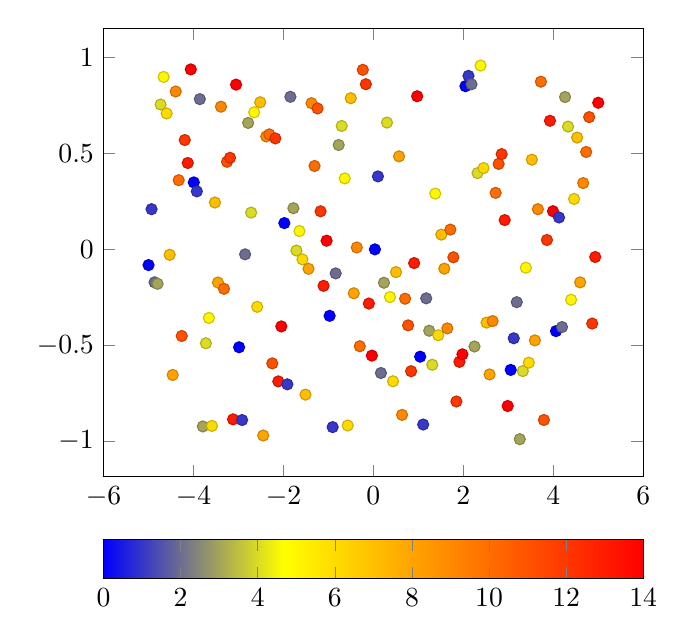
\begin{tikzpicture}
      \begin{axis}[colorbar horizontal]
        \addplot[only marks,scatter,
          scatter src={mod(\coordindex,15)},samples=150]
          {rand};
      \end{axis}
  \end{tikzpicture}}

\end{frame}


\subsection{Testing with EvoSuite}

% SLIDE: Introduction SBST Testing
%!TEX root=kapfhammer_gatorday2015_presentation.tex
% mainfile: ../kapfhammer_gatorday2015_presentation.tex

\begin{frame}[t]

  \frametitle{Search-Based Testing}
  \framesubtitle{Use a fitness function to guide the search to ``good'' values}

  \vspace*{.25in}
  \hspace{.25in}
  \resizebox{3.5in}{!}{
    \begin{tikzpicture}
      \begin{axis}[
          domain=0:1,
          xmax=1,
          ymax=1,
        ]
        \addplot3[surf] {x*y};
        \addplot3[solarizedRebase0,/pgfplots/quiver,
            quiver/u=y,
            quiver/v=x,
            quiver/w=0,
            quiver/scale arrows=0.1,
          -stealth,samples=10] {1};
      \end{axis}
  \end{tikzpicture}}

\end{frame}


% SLIDE: Introduction Mutation Testing
%!TEX root=kapfhammer_gcc_presentation.tex
% mainfile: ../kapfhammer_gcc_presentation.tex

\begin{frame}[t]

  \frametitle{Mutation Testing}
  \framesubtitle{Let's purposefully insert faults into the program under test!}


  \hspace*{-.5in}
  \begin{minipage}{5in}
  \begin{center}

    \begin{minipage}{4.5in}
      \tikzstyle{proc} = [draw, thick, fill=solarizedViolet, text centered, rounded corners,
    text=solarizedRebase02, draw=solarizedViolet]

\tikzstyle{prochighlight} = [draw, thick, fill=solarizedOrange, text centered, rounded corners,
    text=solarizedRebase02, draw=solarizedOrange]

\tikzstyle{procold} = [draw, thick, fill=solarizedViolet!75, text centered, rounded corners,
    text=solarizedRebase02, draw=solarizedViolet!75]

\tikzstyle{procchanged} = [draw, thick, fill=solarizedViolet!75, text centered, rounded corners,
    text=solarizedRebase02, draw=solarizedViolet!75]

\tikzstyle{prochighlightold} = [draw, thick, fill=solarizedOrange!75, text centered, rounded corners,
    text=solarizedRebase02, draw=solarizedOrange!75]

\tikzstyle{prochighlightchanged} = [draw, thick, fill=solarizedYellow!75, text centered, rounded corners,
    text=solarizedRebase02, draw=solarizedYellow!75]

\tikzstyle{proctest} = [draw, thick, fill=solarizedOrange, text centered, rounded corners,
text=solarizedBase02, draw=solarizedOrange]

\tikzstyle{procnew} = [draw, thick, fill=solarizedGreen, text centered, rounded corners,
    text=solarizedRebase02, draw=solarizedGreen]

\tikzstyle{procyellow} = [draw, thick, fill=solarizedYellow, text centered, rounded corners,
    text=solarizedRebase02, draw=solarizedYellow]

\tikzstyle{procred} = [draw, thick, fill=solarizedRed, text centered, rounded corners,
    text=solarizedRebase02, draw=solarizedRed]

\tikzstyle{io} = [ellipse, draw, thick, fill=solarizedBlue, draw=solarizedBlue, text=solarizedRebase02]

\tikzstyle{iopass} = [ellipse, draw, thick, fill=solarizedGreen, draw=solarizedGreen, text=solarizedRebase02]
\tikzstyle{iofail} = [ellipse, draw, thick, fill=solarizedRed, draw=solarizedRed, text=solarizedRebase02]
\tikzstyle{iohighlight} = [ellipse, draw, thick, fill=solarizedYellow, draw=solarizedYellow,
    text=solarizedRebase02]

\tikzstyle{iofailother} = [ellipse, draw, thick, fill=solarizedYellow, draw=solarizedYellow,
    text=solarizedRebase02]
\tikzstyle{wrongoutput} = [ellipse, draw, thick, fill=solarizedCyan, draw=solarizedCyan, text=solarizedRebase02]

\tikzstyle{special} = [draw, thick, fill=solarizedGreen, text centered, draw=solarizedGreen,
    text=solarizedBase02]
\tikzstyle{specialOrange} = [draw, thick, fill=solarizedOrange, text centered, draw=solarizedOrange,
    text=solarizedBase02]
\tikzstyle{specialGreen} = [draw, thick, fill=solarizedGreen, text centered, draw=solarizedGreen,
    text=solarizedBase02]
\tikzstyle{specialYellow} = [draw, thick, fill=solarizedYellow, text centered, draw=solarizedYellow,
    text=solarizedBase02]

\tikzstyle{pass} = [draw, thick, fill=solarizedGreen, text centered, draw=solarizedGreen, text=solarizedRebase02]
\tikzstyle{fail} = [draw, thick, fill=solarizedRed, text centered, draw=solarizedRed, text=solarizedRebase02]

\tikzstyle{feature} = [draw, thick, fill=solarizedOrange, text centered, text=solarizedRebase02, draw=solarizedOrange]


    \begin{figure}

    \begin{center}

      \begin{tikzpicture}[node distance=1cm, auto,>=stealth, thick]

        \path[use as bounding box] (-2,4.35) rectangle (10,-2);

%% 10 test cases, 12 requirements
%% Test case timings (used by Greedy): 5,6,4,2,8,10,4,1,3,2
%% Covers relationships:
%%   T1 = {R1,R2,R3}
%%   T2 = {R2,R3,R4}
%%   T3 = {R1,R5}
%%   T4 = {R4,R6}
%%   T5 = {R5,R6,R7}
%%   T6 = {R6,R7,R8,R9}
%%   T7 = {R7,R8}
%%   T8 = {R8,R10}
%%   T9 = {R9,R12}
%%   T10 = {R10,R11}

        %%%%% 1

        % A Test Case
        \path[->]<1-> node[proc, text width=3ex]
        (One) at (-1.65,2.00) {$T_1$};

        % A Test Case
        \path[->]<1-> node[proc, right of=One,
                      yshift=0in, xshift=.1in, text width=3ex]
                      (Two) {$T_2$};

        % A Test Case
        \path[->]<2-> node[proc, right of=Two,
                      yshift=0in, xshift=.1in, text width=3ex]
                      (Three) {$T_3$};

        % A Test Case
        \path[->]<2-> node[proc, right of=Three,
                      yshift=0in, xshift=.1in, text width=3ex]
                      (Four) {$T_4$};

        % A Test Case
        \path[->]<3-> node[proc, right of=Four,
                      yshift=0in, xshift=.1in, text width=3ex]
                      (Five) {$T_5$};

        % A Test Case
        \path[->]<3-> node[proc, right of=Five,
                      yshift=0in, xshift=.1in, text width=3ex]
                      (Six) {$T_6$};

        % A Test Case
        \path[->]<4-> node[proc, right of=Six,
                      yshift=0in, xshift=.1in, text width=3ex]
                      (Seven) {$T_7$};

        % A Test Case
        \path[->]<4-> node[proc, right of=Seven,
                      yshift=0in, xshift=.1in, text width=3ex]
                      (Eight) {$T_8$};

        % A Test Case
        \path[->]<5-> node[proc, right of=Eight,
                      yshift=0in, xshift=.1in, text width=3ex]
                      (Nine) {$T_9$};

        % A Test Case
        \path[->]<5-> node[proc, right of=Nine,
                      yshift=0in, xshift=.1in, text width=3ex]
                      (Ten) {$T_{10}$};

        % Show the test suite
        \path[->]<6-> node[special, above of=Five,
                      yshift=.1in, xshift=.25in]
                      (TestSuite)
              {Test Suite $T = \langle T_1, T_2, \ldots, T_9, T_{10} \rangle$};

%% 10 test cases, 12 requirements
%% Test case timings (used by Greedy): 5,6,4,2,8,10,4,1,3,2
%% Covers relationships:
%%   T1 = {R1,R2,R3}
%%   T2 = {R2,R3,R4}
%%   T3 = {R1,R5}
%%   T4 = {R4,R6}
%%   T5 = {R5,R6,R7}
%%   T6 = {R6,R7,R8,R9}
%%   T7 = {R7,R8}
%%   T8 = {R8,R10}
%%   T9 = {R9,R12}
%%   T10 = {R10,R11}

        %%%%% 2

        \path[->]<7-> node[prochighlight, text width=3ex]
        (OneR) at (-1.825,-1.00) {$M_1$};

        \path[->]<7-> node[prochighlight, right of=OneR,
                      yshift=0in, xshift=.02in, text width=3ex]
                      (TwoR) {$M_2$};

        \path[->]<8-> node[prochighlight, right of=TwoR,
                      yshift=0in, xshift=.02in, text width=3ex]
                      (ThreeR) {$M_3$};

        \path[->]<8-> node[prochighlight, right of=ThreeR,
                      yshift=0in, xshift=.02in, text width=3ex]
                      (FourR) {$M_4$};

        \path[->]<9-> node[prochighlight, right of=FourR,
                      yshift=0in, xshift=.02in, text width=3ex]
                      (FiveR) {$M_5$};

        \path[->]<9-> node[prochighlight, right of=FiveR,
                      yshift=0in, xshift=.02in, text width=3ex]
                      (SixR) {$M_6$};

        \path[->]<10-> node[prochighlight, right of=SixR,
                      yshift=0in, xshift=.02in, text width=3ex]
                      (SevenR) {$M_7$};

        \path[->]<10-> node[prochighlight, right of=SevenR,
                      yshift=0in, xshift=.02in, text width=3ex]
                      (EightR) {$M_8$};

        \path[->]<11-> node[prochighlight, right of=EightR,
                      yshift=0in, xshift=.02in, text width=3ex]
                      (NineR) {$M_9$};

        \path[->]<11-> node[prochighlight, right of=NineR,
                      yshift=0in, xshift=.02in, text width=3ex]
                      (TenR) {$M_{10}$};

        \path[->]<12-> node[prochighlight, right of=TenR,
                      yshift=0in, xshift=.02in, text width=3ex]
                      (ElevenR) {$M_{11}$};

        \path[->]<12-> node[prochighlight, right of=ElevenR,
                      yshift=0in, xshift=.02in, text width=3ex]
                      (TwelveR) {$M_{12}$};

%% 10 test cases, 12 requirements
%% Test case timings (used by Greedy): 5,6,4,2,8,10,4,1,3,2
%% Covers relationships:
%%   T1 = {R1,R2,R3}
%%   T2 = {R2,R3,R4}
%%   T3 = {R1,R5}
%%   T4 = {R4,R6}
%%   T5 = {R5,R6,R7}
%%   T6 = {R6,R7,R8,R9}
%%   T7 = {R7,R8}
%%   T8 = {R8,R10}
%%   T9 = {R9,R12}
%%   T10 = {R10,R11}

        %%%%% 3

        % Show the set of requirements
        \path[->]<13-> node[special, below of=SixR,
                      yshift=-.1in, xshift=.25in]
                      (Requirements)
              {Set of Program Methods $M = \{ M_1, M_2, \ldots, M_{11}, M_{12} \}$};

        %%%%% 4

        \path[->]<14-> node[prochighlight, right of=ElevenR,
                      yshift=0in, xshift=.02in, text width=3ex]
                      (TwelveR) {$M_{12}$}
        (One) edge node {} (OneR)
        (One) edge node {} (TwoR)
        (One) edge node {} (FourR);

        \path[->]<14-> node[prochighlight, right of=ElevenR,
                      yshift=0in, xshift=.02in, text width=3ex]
                      (TwelveR) {$M_{12}$}
        (Two) edge node {} (TwoR)
        (Two) edge node {} (ThreeR)
        (Two) edge node {} (FourR);

        \path[->]<14-> node[prochighlight, right of=ElevenR,
                      yshift=0in, xshift=.02in, text width=3ex]
                      (TwelveR) {$M_{12}$}
        (Three) edge node {} (OneR)
        (Three) edge node {} (FiveR);

        \path[->]<14-> node[prochighlight, right of=ElevenR,
                      yshift=0in, xshift=.02in, text width=3ex]
                      (TwelveR) {$M_{12}$}
        (Four) edge node {} (FourR)
        (Four) edge node {} (SixR);

        \path[->]<15-> node[prochighlight, right of=ElevenR,
                      yshift=0in, xshift=.02in, text width=3ex]
                      (TwelveR) {$M_{12}$}
        (Five) edge node {} (FiveR)
        (Five) edge node {} (SixR)
        (Five) edge node {} (SevenR);

        \path[->]<15-> node[prochighlight, right of=ElevenR,
                      yshift=0in, xshift=.02in, text width=3ex]
                      (TwelveR) {$M_{12}$}
        (Six) edge node {} (SixR)
        (Six) edge node {} (SevenR)
        (Six) edge node {} (EightR)
        (Six) edge node {} (NineR);

        \path[->]<16-> node[prochighlight, right of=ElevenR,
                      yshift=0in, xshift=.02in, text width=3ex]
                      (TwelveR) {$M_{12}$}
        (Seven) edge node {} (SevenR)
        (Seven) edge node {} (EightR);

        \path[->]<16-> node[prochighlight, right of=ElevenR,
                      yshift=0in, xshift=.02in, text width=3ex]
                      (TwelveR) {$M_{12}$}
        (Eight) edge node {} (EightR)
        (Eight) edge node {} (TenR);

        \path[->]<16-> node[prochighlight, right of=ElevenR,
                      yshift=0in, xshift=.02in, text width=3ex]
                      (TwelveR) {$M_{12}$}
        (Nine) edge node {} (NineR)
        (Nine) edge node {} (TwelveR);

        \path[->]<16-> node[prochighlight, right of=ElevenR,
                      yshift=0in, xshift=.02in, text width=3ex]
                      (TwelveR) {$M_{12}$}
        (Ten) edge node {} (TenR)
        (Ten) edge node {} (ElevenR);

        % FINAL PART WHERE WE EITHER FIND OR DO NOT FIND THE FAULT

        \path[->]<17-18> node[procyellow, right of=ThreeR,
                      yshift=0in, xshift=.02in, text width=3ex]
                      (FourR) {$M_4$};

        % A Test Case
        \path[->]<18-18> node[procred, text width=3ex]
        (One) at (-1.65,2.00) {$T_1$};

        \path[->]<19-> node[prochighlight, right of=ThreeR,
                      yshift=0in, xshift=.02in, text width=3ex]
                      (FourR) {$M_4$};

        % A Test Case
        \path[->]<19-> node[proc, text width=3ex]
        (One) at (-1.65,2.00) {$T_1$};

        \path[->]<20-> node[procyellow, right of=SevenR,
                      yshift=0in, xshift=.02in, text width=3ex]
                      (EightR) {$M_8$};

        \end{tikzpicture}

        \end{center}

        \end{figure}

      \end{minipage}

  \end{center}
  \end{minipage}

\end{frame}


% SLIDE: Explain the basics of EvoSuite
%!TEX root=kapfhammer_gatorday2015_presentation.tex
% mainfile: kapfhammer_gatorday2015_presentation.tex

\begin{frame}[t]
  \frametitle{Testing with EvoSuite}
  \framesubtitle{This prototype can automatically generate real JUnit test suites!}

  \hspace*{-.5in}
  \begin{minipage}{5in}
  \begin{center}

    \begin{minipage}{4.5in}

    \tikzstyle{proc} = [draw, thick, fill=solarizedViolet, text centered, rounded corners,
    text=solarizedRebase02, draw=solarizedViolet]

\tikzstyle{prochighlight} = [draw, thick, fill=solarizedOrange, text centered, rounded corners,
    text=solarizedRebase02, draw=solarizedOrange]

\tikzstyle{procold} = [draw, thick, fill=solarizedViolet!75, text centered, rounded corners,
    text=solarizedRebase02, draw=solarizedViolet!75]

\tikzstyle{procchanged} = [draw, thick, fill=solarizedViolet!75, text centered, rounded corners,
    text=solarizedRebase02, draw=solarizedViolet!75]

\tikzstyle{prochighlightold} = [draw, thick, fill=solarizedOrange!75, text centered, rounded corners,
    text=solarizedRebase02, draw=solarizedOrange!75]

\tikzstyle{prochighlightchanged} = [draw, thick, fill=solarizedYellow!75, text centered, rounded corners,
    text=solarizedRebase02, draw=solarizedYellow!75]

\tikzstyle{proctest} = [draw, thick, fill=solarizedOrange, text centered, rounded corners,
text=solarizedBase02, draw=solarizedOrange]

\tikzstyle{procnew} = [draw, thick, fill=solarizedGreen, text centered, rounded corners,
    text=solarizedRebase02, draw=solarizedGreen]

\tikzstyle{procyellow} = [draw, thick, fill=solarizedYellow, text centered, rounded corners,
    text=solarizedRebase02, draw=solarizedYellow]

\tikzstyle{procred} = [draw, thick, fill=solarizedRed, text centered, rounded corners,
    text=solarizedRebase02, draw=solarizedRed]

\tikzstyle{io} = [ellipse, draw, thick, fill=solarizedBlue, draw=solarizedBlue, text=solarizedRebase02]

\tikzstyle{iopass} = [ellipse, draw, thick, fill=solarizedGreen, draw=solarizedGreen, text=solarizedRebase02]
\tikzstyle{iofail} = [ellipse, draw, thick, fill=solarizedRed, draw=solarizedRed, text=solarizedRebase02]
\tikzstyle{iohighlight} = [ellipse, draw, thick, fill=solarizedYellow, draw=solarizedYellow,
    text=solarizedRebase02]

\tikzstyle{iofailother} = [ellipse, draw, thick, fill=solarizedYellow, draw=solarizedYellow,
    text=solarizedRebase02]
\tikzstyle{wrongoutput} = [ellipse, draw, thick, fill=solarizedCyan, draw=solarizedCyan, text=solarizedRebase02]

\tikzstyle{special} = [draw, thick, fill=solarizedGreen, text centered, draw=solarizedGreen,
    text=solarizedBase02]
\tikzstyle{specialOrange} = [draw, thick, fill=solarizedOrange, text centered, draw=solarizedOrange,
    text=solarizedBase02]
\tikzstyle{specialGreen} = [draw, thick, fill=solarizedGreen, text centered, draw=solarizedGreen,
    text=solarizedBase02]
\tikzstyle{specialYellow} = [draw, thick, fill=solarizedYellow, text centered, draw=solarizedYellow,
    text=solarizedBase02]

\tikzstyle{pass} = [draw, thick, fill=solarizedGreen, text centered, draw=solarizedGreen, text=solarizedRebase02]
\tikzstyle{fail} = [draw, thick, fill=solarizedRed, text centered, draw=solarizedRed, text=solarizedRebase02]

\tikzstyle{feature} = [draw, thick, fill=solarizedOrange, text centered, text=solarizedRebase02, draw=solarizedOrange]


    \begin{figure}

    \begin{center}

      \begin{tikzpicture}[node distance=0cm, auto,>=stealth, thick]

        \path[use as bounding box] (-2,4.5) rectangle (10,-2);

        % Computer Software
        \path[->]<1-> node[proc, text width=14ex]
        (Software) at (4,.8) {Evolutionary Testing};

        % Code
        \path[->]<2-> node[proc, right of=Software,
                      yshift=-.5in, xshift=-1.75in, text width=14ex]
                      (Code) {Representation}
        (Software) edge node {} (Code);

        % Features
        \path[->]<3-> node[proc, below of=Software,
                      yshift=-1in, xshift=-.75in, text width=12ex]
                      (Features) {Fitness \\ Function}
        (Software) edge node {} (Features);

        % Feature Interactions
        \path[->]<4-> node[proc, below of=Software,
                      yshift=-1in, xshift=.75in, text width=12ex]
                      (Interactions) {Modify \\ Program}
        (Software) edge node {} (Interactions);

        % Execution Environments
        \path[->]<5-> node[proc, right of=Software,
                      yshift=-.5in, xshift=1.75in, text width=12ex]
                      (Environment) {Operators}
        (Software) edge node {} (Environment);

        % Brooks Quotation
        \path[->]<6-> node[specialOrange, above of=Software,
                      yshift=.8in,text width=40ex]
                      (Quotations)
                      {``1600 Faults in 100 Projects: Automatically Finding Faults While Achieving High Coverage with
                      EvoSuite'', {\em Empirical Software Engineering}};

        \end{tikzpicture}

        \end{center}

        \end{figure}

      \end{minipage}

  \end{center}
  \end{minipage}


\end{frame}



% SLIDE: Explain the EvoSuite methods
%!TEX root=kapfhammer_gatorday2015_presentation.tex
% mainfile: kapfhammer_gatorday2015_presentation.tex

\begin{frame}[t]
  \frametitle{Configuring EvoSuite}
  \framesubtitle{This tool has many unique configurations --- which are best?}

  \hspace*{-.5in}
  \begin{minipage}{5in}
  \begin{center}
  \vspace*{.1in}

    \begin{minipage}{4.5in}

    \tikzstyle{proc} = [draw, thick, fill=solarizedViolet, text centered, rounded corners,
    text=solarizedRebase02, draw=solarizedViolet]

\tikzstyle{prochighlight} = [draw, thick, fill=solarizedOrange, text centered, rounded corners,
    text=solarizedRebase02, draw=solarizedOrange]

\tikzstyle{procold} = [draw, thick, fill=solarizedViolet!75, text centered, rounded corners,
    text=solarizedRebase02, draw=solarizedViolet!75]

\tikzstyle{procchanged} = [draw, thick, fill=solarizedViolet!75, text centered, rounded corners,
    text=solarizedRebase02, draw=solarizedViolet!75]

\tikzstyle{prochighlightold} = [draw, thick, fill=solarizedOrange!75, text centered, rounded corners,
    text=solarizedRebase02, draw=solarizedOrange!75]

\tikzstyle{prochighlightchanged} = [draw, thick, fill=solarizedYellow!75, text centered, rounded corners,
    text=solarizedRebase02, draw=solarizedYellow!75]

\tikzstyle{proctest} = [draw, thick, fill=solarizedOrange, text centered, rounded corners,
text=solarizedBase02, draw=solarizedOrange]

\tikzstyle{procnew} = [draw, thick, fill=solarizedGreen, text centered, rounded corners,
    text=solarizedRebase02, draw=solarizedGreen]

\tikzstyle{procyellow} = [draw, thick, fill=solarizedYellow, text centered, rounded corners,
    text=solarizedRebase02, draw=solarizedYellow]

\tikzstyle{procred} = [draw, thick, fill=solarizedRed, text centered, rounded corners,
    text=solarizedRebase02, draw=solarizedRed]

\tikzstyle{io} = [ellipse, draw, thick, fill=solarizedBlue, draw=solarizedBlue, text=solarizedRebase02]

\tikzstyle{iopass} = [ellipse, draw, thick, fill=solarizedGreen, draw=solarizedGreen, text=solarizedRebase02]
\tikzstyle{iofail} = [ellipse, draw, thick, fill=solarizedRed, draw=solarizedRed, text=solarizedRebase02]
\tikzstyle{iohighlight} = [ellipse, draw, thick, fill=solarizedYellow, draw=solarizedYellow,
    text=solarizedRebase02]

\tikzstyle{iofailother} = [ellipse, draw, thick, fill=solarizedYellow, draw=solarizedYellow,
    text=solarizedRebase02]
\tikzstyle{wrongoutput} = [ellipse, draw, thick, fill=solarizedCyan, draw=solarizedCyan, text=solarizedRebase02]

\tikzstyle{special} = [draw, thick, fill=solarizedGreen, text centered, draw=solarizedGreen,
    text=solarizedBase02]
\tikzstyle{specialOrange} = [draw, thick, fill=solarizedOrange, text centered, draw=solarizedOrange,
    text=solarizedBase02]
\tikzstyle{specialGreen} = [draw, thick, fill=solarizedGreen, text centered, draw=solarizedGreen,
    text=solarizedBase02]
\tikzstyle{specialYellow} = [draw, thick, fill=solarizedYellow, text centered, draw=solarizedYellow,
    text=solarizedBase02]

\tikzstyle{pass} = [draw, thick, fill=solarizedGreen, text centered, draw=solarizedGreen, text=solarizedRebase02]
\tikzstyle{fail} = [draw, thick, fill=solarizedRed, text centered, draw=solarizedRed, text=solarizedRebase02]

\tikzstyle{feature} = [draw, thick, fill=solarizedOrange, text centered, text=solarizedRebase02, draw=solarizedOrange]


    \begin{figure}

    \begin{center}

      \begin{tikzpicture}[node distance=0cm, auto,>=stealth, thick]

        \path[use as bounding box] (-2,4.5) rectangle (10,-2);

        % Computer Software
        \path[->]<1-> node[proc, text width=14ex]
        (Software) at (4,.8) {EvoSuite's Configurations};

        % Code
        \path[->]<2-> node[proc, right of=Software,
                      yshift=-.5in, xshift=-1.75in, text width=12ex]
                      (Code) {Random}
        (Software) edge node {} (Code);

        % Features
        \path[->]<3-> node[proc, below of=Software,
                      yshift=-1in, xshift=-.75in, text width=14ex]
                      (Features) {Fixed-Random}
        (Software) edge node {} (Features);

        % Feature Interactions
        \path[->]<4-> node[proc, below of=Software,
                      yshift=-1in, xshift=.75in, text width=12ex]
                      (Interactions) {Genetic}
        (Software) edge node {} (Interactions);

        % Execution Environments
        \path[->]<5-> node[proc, right of=Software,
                      yshift=-.5in, xshift=1.75in, text width=12ex]
                      (Environment) {Regression}
        (Software) edge node {} (Environment);

        % Brooks Quotation
        \path[->]<6-> node[specialOrange, above of=Software,
                      yshift=.8in,text width=40ex]
                      (Quotations)
                      {The fitness function computes {\em branch coverage}, {\em weak mutation score}, or {\em strong
                      mutation score} to guide the search to the ``best'' test cases};

        \end{tikzpicture}

        \end{center}

        \end{figure}

      \end{minipage}

  \end{center}
  \end{minipage}


\end{frame}



% SLIDE: Show a Test Case Generated by EvoSuite
%!TEX root=kapfhammer_gcc_presentation.tex
% mainfile: ../kapfhammer_gcc_presentation.tex

\begin{frame}[fragile]
  \frametitle{\vspace*{.5in}A Test from EvoSuite}
  \framesubtitle{}

  \normalsize
  \hspace*{-.75in}
  \begin{minipage}{5in}
    \large
    \vspace*{-.25in}
    \begin{minted}{java}

      @Test
      public void test001() throws Throwable {
        int int0 = 0;
        String string0 = Kinetic.computeVelocity(int0, int0);
        assertEquals("Undefined", string0);
        assertNotNull(string0);
        int int1 = 1262;
        String string1 = Kinetic.computeVelocity(int0, int0);
        int int2 = 5349;
        String string2 = Kinetic.computeVelocity(int1, int2);
        int int3 = 0;
        int int4 = 3;
        String string3 = Kinetic.computeVelocity(int3, int4);
        Kinetic kinetic0 = new Kinetic();
      }

    \end{minted}
  \end{minipage}
  \normalsize

\end{frame}


% SLIDE: Ask some questions about the use of EvoSuite
%!TEX root=kapfhammer_gcc_presentation.tex
% mainfile: ../kapfhammer_gcc_presentation.tex

\begin{frame}[t]

  \frametitle{Important Questions}
  \framesubtitle{EvoSuite is an advanced, yet sometimes limited, testing tool}

  \begin{tikzpicture}[overlay, remember picture]
    \node[anchor=center] at (current page.center) {
        \begin{beamercolorbox}[center]{title}
          \vspace*{.4in}
          \fontsize{30}{40}\selectfont
          \begin{center}
            \only<1>{\vspace*{.2in} Will EvoSuite's test cases find the fault in the example program?}
            \only<2>{What is missing from the test cases that EvoSuite generates?}
            \only<3>{\vspace*{.2in}How does the {\em oracle problem} influence the effectiveness of EvoSuite?}
            \only<4>{\vspace*{.2in}What are the {\em fundamental} limitations of automated testing?}
          \end{center}
          \normalsize
      \end{beamercolorbox}};
  \end{tikzpicture}

\end{frame}


% SLIDE: Introduce the NSB hypothesis
%!TEX root=kapfhammer_gatorday2015_presentation.tex
% mainfile: ../kapfhammer_gatorday2015_presentation.tex

\begin{frame}[t]

  \frametitle{No Silver Bullet}
  \framesubtitle{Software tools are fundamentally limited --- what is our hope?}

  \begin{tikzpicture}[overlay, remember picture]
    \node[anchor=center] at (current page.center) {
        \begin{beamercolorbox}[center]{title}
          \vspace*{.8in}
          \Large
          \begin{center}
            \begin{quote}
              There is no single development, in either technology or management technique, which by itself promises even
              one order-of-magnitude improvement within a decade in productivity, in reliability, in simplicity. \\ \vspace*{.1in}
              {\color{solarizedViolet}{\em Frederick P.\ Brooks, Jr.}, Proceedings of the IFIP Tenth World Computing
              Conference, {\em 1986}}
            \end{quote}
          \end{center}
          \normalsize
      \end{beamercolorbox}};
  \end{tikzpicture}

\end{frame}














%%%%%%%%%%%%%%%%%%%%%%%%%%%%%
% Search-Based Software Testing
%%%%%%%%%%%%%%%%%%%%%%%%%%%%%

\section{Conclusion}
\label{sec:conclusion}
%!TEX root=kapfhammer_gcc_presentation.tex
% mainfile: kapfhammer_gcc_presentation.tex

% SLIDE: Table of contents
%!TEX root=kapfhammer_gcc_presentation.tex
% mainfile: ../kapfhammer_gcc_presentation.tex

\begin{frame}

  % \frametitle{\vspace*{.5in}{
  % {\fontsize{22}{0}\selectfont``Searching'' for the Best Tests}}}
  % \framesubtitle{An introduction to automated software testing with search-based techniques}

  \vspace*{.15in}
  \tableofcontents[
  pausesections,
  currentsection,
  % currentsubsection,
  sectionstyle=show/shaded,
  % subsectionstyle=show/shaded,
  ]
\end{frame}



% SLIDE: The need for great designers
% %!TEX root=kapfhammer_gatorday2015_presentation.tex
% mainfile: ../kapfhammer_gatorday2015_presentation.tex

\setbeamertemplate{bibliography item}{\cmark \hspace*{-1in}}
\begin{frame}
  \frametitle{Further Resources}
  \framesubtitle{Read these papers and/or contact me if you want to learn more!}

    \raggedright
    \nocite{*}
    \printbibliography
    % \bibliography{bibliography}

\end{frame}


% SLIDE: The need for great designers
%!TEX root=kapfhammer_gcc_presentation.tex
% mainfile: ../kapfhammer_gcc_presentation.tex

\begin{frame}[t]
  \frametitle{The Software Crisis}
  \framesubtitle{Solutions are available --- but not always obvious or popular}

  \begin{tikzpicture}[overlay, remember picture]
    \node[anchor=center] at (current page.center) {
        \begin{beamercolorbox}[center]{title}
          \vspace*{.4in}
          \fontsize{30}{40}\selectfont
          \begin{center}
            \only<1>{What are the solutions to the \hspace*{.25in} software crisis?}
            \only<2>{\fontsize{50}{60}\selectfont \hspace*{-.45in} Great Designers}
            \only<3>{\fontsize{50}{60}\selectfont Unremitting Care}
            \only<4>{\fontsize{50}{60}\selectfont Incremental Advances}
          \end{center}
          \normalsize
      \end{beamercolorbox}};
  \end{tikzpicture}

\end{frame}


% SLIDE: The final slide
%!TEX root=kapfhammer_gcc_presentation.tex
% mainfile: ../kapfhammer_gcc_presentation.tex

\begin{frame}[t]
  \frametitle{Final Admonishment}
  \framesubtitle{An epilogue called ``Fifty Years of Wonder, Excitement, and Joy''}

  \begin{tikzpicture}[overlay, remember picture]
    \node[anchor=center] at (current page.center) {
        \begin{beamercolorbox}[center]{title}
          \vspace*{.8in}
          \Large
          \begin{center}
            \begin{quote}
              Too many interests, too many exciting opportunities for learning, research, and thought. What a marvelous
              predicament! Not only is the end not in sight, but the pace is not slackening. {\color{solarizedYellow}We
              have many future joys.}
              \\ \vspace*{.1in}
              {\color{solarizedViolet}{\em Frederick P.\ Brooks, Jr.}, The Mythical Man-Month, {\em 1995}}
            \end{quote}
          \end{center}
          \normalsize
      \end{beamercolorbox}};
  \end{tikzpicture}

\end{frame}


% SLIDE: The final slide
%!TEX root=kapfhammer_gatorday2015_presentation.tex
% mainfile: ../kapfhammer_gatorday2015_presentation.tex

\begin{frame}[t]
  \frametitle{Evaluation }
  \framesubtitle{Please provide your evaluation and assess your learning.}

  \begin{minipage}{5in}
  \begin{tikzpicture}[overlay, remember picture]
    \node[anchor=center] at (current page.center) {
        \begin{beamercolorbox}[center]{title}
          \vspace*{.6in}
          \fontsize{30}{40}\selectfont
          \begin{center}
            \includegraphics[scale=15.0]{images/qrcode.png} \\ 
            \vspace*{-.2in}
            \url{http://goo.gl/iJu0wq}
          \end{center}
          \normalsize
      \end{beamercolorbox}};
  \end{tikzpicture}
  \end{minipage}

\end{frame}



% \begin{frame}
%   \titlepage
% \end{frame}

\end{document}
